
\documentclass[letterpaper]{vldb}

\usepackage{graphicx}
\usepackage{balance}
\usepackage{xspace}

\usepackage{times}
\usepackage{color}

\usepackage{algorithm}
\usepackage{algorithmic}
\renewcommand{\algorithmicrequire}{\textbf{Input:}}
\renewcommand{\algorithmicensure}{\textbf{Output:}}

\newcommand{\eml}{\texttt{ease.ml}\xspace}

\newtheorem{theorem}{Theorem}
\newtheorem{conjecture}[theorem]{Conjecture}
\newtheorem{lemma}[theorem]{Lemma}
\newtheorem{claim}[theorem]{Claim}
\newtheorem{observation}[theorem]{Observation}
\newtheorem{corollary}[theorem]{Corollary}
\newtheorem{example}[theorem]{Example}
\newtheorem{condition}[theorem]{Condition}
\newtheorem{definition}[theorem]{Definition}
\newtheorem{proposition}[theorem]{Proposition}

\newcommand{\cA}{\mathcal{A}}

\newcommand{\cN}{\mathcal{N}}
\newcommand{\cV}{\mathcal{V}}
\newcommand{\cU}{\mathcal{U}}
%\newcommand{\cA}{\mathcal{A}}
\newcommand{\cM}{\mathcal{M}}
\newcommand{\cD}{\mathcal{D}}
\newcommand{\cE}{\mathcal{E}}
\newcommand{\cL}{\mathcal{L}}
\newcommand{\cJ}{\mathcal{J}}
\newcommand{\cP}{\mathcal{P}}
\newcommand{\cF}{\mathcal{F}}
\newcommand{\cH}{\mathcal{H}}
\newcommand{\cS}{\mathcal{S}}
\newcommand{\C}{\mathbb{C}}
\newcommand{\bH}{\mathbb{H}}
\newcommand{\bL}{\mathbb{L}}
\newcommand{\E}{\mathbb{E}}
\newcommand{\F}{\mathbb{F}}
\newcommand{\V}{\mathbb{V}}
\newcommand{\N}{\mathbb{N}}
\newcommand{\bP}{\mathbb{P}} % \P is used by the system
\newcommand{\ds}{\displaystyle}



\def\R{\mathbb{R}}


\DeclareMathOperator*{\argmin}{arg\,min}
\DeclareMathOperator*{\argmax}{arg\,max}
\DeclareMathOperator{\SYN}{SYN}


\begin{document}

%\title{Towards Multi-tenant Machine Learning Infrastructures}
%\title{Towards ``Machine Learning as a Service'': \\
%The Multi-tenant Case}


\title{Multi-tenant Model Selection in ease.ml}
%: \\
%Towards ``Machine Learning as a Service''}

\author{
XXX~~~~~XXX~~~~~XXX~~~~~XXX~~~~~XXX~~~~~XXX\\
XXX~~~~~XXX~~~~~XXX~~~~~XXX~~~~~XXX~~~~~XXX\\
XXX~~~~~XXX~~~~~XXX~~~~~XXX~~~~~XXX~~~~~XXX\\
XXX~~~~~XXX~~~~~XXX~~~~~XXX~~~~~XXX~~~~~XXX
}

\maketitle

\begin{abstract}
We present \eml, a \emph{declarative} machine learning service platform we build
to support more than ten research groups outside the computer science departments at ETH Zurich 
for their machine learning needs.
With \eml, user defines the high-level 
schema of a machine learning application, submits
the task via a Web interface, and the system automatically deals with the rest, such as model selection and data movement.
In this paper, we describe the \eml architecture and focus on
a novel technical problem introduced by \eml regarding resource allocation.
We ask, {\em as a ``service provider'' who manages a shared cluster of 
machines among all of our users running machine learning workloads, what is the resource
allocation strategy that maximizes the global happiness of all
of our users?}


%From a single user's perspective, \eml is not
%dissimilar to a declarative
%machine learning, or ``AutoML'', system that provides 
%automatic support
%for model selection and hyperparameter tuning.


Resource allocation is a critical yet subtle issue in this multi-tenant scenario, as we have to balance between efficiency and fairness.
We provide the first formalization of the problem that we call {\em multi-tenant model selection}, aiming for minimizing the total {\em regrets} of all users
running automatic model selection tasks.
We then develop a novel algorithm that combines multi-armed bandits with Bayesian optimization, and prove, to the best of our knowledge, the first regret bound under the multi-tenant setting.
Finally, we report our evaluation of \eml on both synthetic data and one service we are providing to our users, namely, 
image classification with deep neural networks.
Our experimental evaluation results show that our proposed solution can 
be up to 9.8$\times$ faster to achieve the same global quality
for all users compared with %strong baselines 
two popular heuristics used by our users before \eml.

%
%often by 
%a significant margin.


%
%and (2) structured data classification with
%Azure machine learning studio.
%On these use cases, \eml is able to outperform
%approaches popularly used by
%state-of-the-art resource managers 
%designed for more general workloads by up to XXX$\times$.
\end{abstract} 

%\vspace{-1em}
\section{Introduction}\label{sec:introduction}

Recent decade has witnessed the increasingly 
ubiquitous applications of machine learning techniques 
to areas beyond computer sciences. 
One consequence of these wide applications
is that we can no longer assume a computer science 
background on our users. As a result, how to make
machine learning techniques more {\em accessible} and
{\em usable} to non-computer science users has become
a research topic that attracts intensive interests
from both the database~\cite{XXX,XXX,XXX,XXX,XXX}
and the machine learning community~\cite{XXX,XXX,XXX,XXX,XXX}.

\paragraph*{Motivating Example} At ETH Zurich,
we, as a research group, provide ``data science
services'' to other research groups outside the computer science domain.
These users provide
us their data sets and the tasks they 
want to perform with machine learning; and
we host these data sets on our machines
for our users to run their machine learning
jobs (e.g.,
TensorFlow~\cite{XXX} and Keras~\cite{XXX}).
Although we also have students serving as ``consultants''
to answer users' questions, it is still our
users who run machine learning systems
by themselves in most cases. As of today, our infrastructure
contains 29 TITAN X GPUs and 100 TB storage
shared by more than ten research groups
from areas including astrophysics,
biology, social sciences, meteorology, 
material science, and the university hospital.
In this paper, we ask, {\em what is an
efficient and effective way for multiple users sharing 
the same computational infrastructure running
machine learning tasks?}

\vspace{0.5em}
\noindent
{\bf Failed Experience 1.} Our first strategy was to provide
all users \texttt{ssh} access to all of our machines
and a shared Google Calendar for resource allocation.
However, even when everyone respects the resource allocation
protocol (which rarely happens), our users compete with 
resources fiercely; this decentralized management strategy failed in chaos in just less than two weeks. 

\vspace{0.5em}
\noindent
{\bf Failed Experience 2.} We then resorted to classic resource
managers and used \texttt{Slurm} for users to submit 
their jobs. 
%Each user is assigned with a priority
%and a fixed quota, and the resource manager
%schedules users' job. Only when there are freely
%available resources a user can get resources above 
%her quota. 
Although this strategy isolates
users from competing for resources, it poses a
new problem for effective resource utilization.
In almost all of our applications, the user needs to conduct 
a series of explorations of different machine learning
models.
However, not all these explorations conducted by
our users are necessary (either because of the lack
of machine learning knowledge from our users or automatic 
scripts just conducting exhaustive search). For example,
one of our users used five GPUs for a whole week
trying different models to improve
over a model that already has an accuracy of 0.99.
Another user 
continued to use his resources trying deeper and 
deeper neural networks even though much simpler
networks already overfit on his dataset.
May these resources be allocated to other users,
they would make much better use of the computation time.

\vspace{0.5em}
Motivated by these experiences, we design
\eml, an automatic resource manager for multi-tenant machine learning workloads.
Compared with existing multi-tenant 
resource managers~\cite{XXX,XXX,XXX,XXX,XXX,XXX,XXX,XXX}, \eml
is aware of the underlying workload and is able to
integrate knowledge about machine learning
to guide the exploration process more effectively.
Specifically, we formalize the resource allocation problem as what we call ``{\em multi-tenant model selection}.''
Compared with existing systems for automatic
model selection~\cite{XXX,XXX,XXX,XXX,XXX,XXX,XXX,XXX}, \eml is aware of the existence of
multiple users and tries to balance and optimize for
the ``global happiness'' of all users.


\paragraph*{Challenges}

Automatic model selection is crucial for declarative machine learning services and has been studied intensively and extensively in the literature.
However, previous studies focus on the ``single-tenant'' case rather than the multi-tenant case when multiple users compete
for resources.
In this paper, we start by adopting a classic 
view point for single-tenant model selection by treating 
it as a \emph{multi-armed bandit} problem. 
The key idea behind a bandit problem is
to balance between between \emph{exploration} and \emph{exploitation}. When extending existing, single-tenant 
bandit-based solutions to the multi-tenant case, 
we face two major challenges:

\noindent
{\bf (Optimization Objective)} The optimization objective for the single-tenant case is well understood: We want to find the best model for the user as soon as possible (i.e., to minimize
  user's {\em regret} accumulated over time).
  The first challenge is to extend this objective for
  multiple users --- simply treating each user 
  independently is not optimal because reducing regret for one user may increase regret for another, at any given time. 
  Therefore, we need to first design a reasonable
  multi-tenant objective and then design novel
  algorithms to balance not only between
  exploration and exploitation, but also
  {\em fairness} and {\em global efficiency}. Moreover,
  we hope that the algorithms we designed should have rigorous
  theoretical guarantee similar to the single-tenant case.
  
\noindent
{\bf (Heterogeneous Costs and Performance)} It is
  common practice for single-tenant model selection
  algorithms to also consider the execution cost of
  a given model. This is important as models with
  vastly different costs may have similar performance 
  on a particular dataset. Therefore, any multi-tenant
  model selection algorithm we propose should also
  be aware of costs. This makes the integration and
  theoretical analysis of costs even more complicated
  than the single-tenant case because models with 
  different costs now may also have different quality for 
  different users. 
  



  %his implies that we have to sacrifice fairness, namely, we cannot ensure uniform regret reduction when multiple users are involved. Based on this observation, we propose to minimize the {\em total} regret for {\em all} users. Intuitively, this is an unfair strategy, as the system will bias towards users with high ``potential'' in terms of the performance improvement of the models they are running. Nevertheless, the system achieves optimal efficiency in resource allocation, as the system always picks the next user with the highest performance improvement. In the long run, this strategy can minimize the total time spent on identifying best models for all users and thus maximize resource utilization at any given time.

\vspace{-1em}
\paragraph*{Summary of Technical Contributions}
To address the above challenges, our solution is a novel
framework for multi-tenant, cost-aware model selection
integrated into \eml, a declarative machine learning
service platform we build for our local collaborators
at ETH Zurich.
We summarize our contributions as follows.

\noindent
{\bf C1. (System Architecture and Problem Formulation)}
To our best knowledge, \eml is the first system of its kind
and our first contribution is the system design and the formulation
of the core technical problem to build \eml. 
\eml's design goal is two fold---(1) provide an abstraction
to enable more effective model exploration for our users, and 
(2) manage the shared infrastructure to enable more efficient
resource utilization of the exploration process 
for {\em all}, instead of, {\em one} of our users.

From user's perspective, \eml provides a simple high-level 
language to our user. In \eml, the user thinks about 
machine learning as a {\em arbitrary function approximator}.
To specify such an approximator, the users provides the
system (1) the size of the input, (2) the size of the output,
and (3) pairs of examples the function aims to approximate.
For example, if the user wants to train a classifier
for RGB images into 3 classes, she would submit a job like
\[
\texttt{Input = [256, 256, 3]
        Output = [3]}.
\]
\eml then automatically matches all {\em consistent} machine
learning models (e.g., AlexNet, ResNet-18, GoogLeNet, etc.) 
that can be used for users' application, and
explore all these models for users. Whenever a new model
finished running, \eml returns the model to the user.
Despite the simplicity of this abstraction, more than 70\% of
our users' applications can be build in this way.

From infrastructure's perspective, \eml then contains an
automatic scheduler to prioritize the execution of
different models for different users. 
We formalize
this as a novel technical problem 
we call {\em multitenant model selection}.

\noindent
{\bf C2. (Multitenant Multi-armed Bandits)} Our second contribution
is to provide the first algorithm for the multitenant model selection
problem. In this paper, we develop a novel family of algorithms by extending 
classic \texttt{GP-UCB} algorithm for a singletenant model
selection to multitenant cases. 
From a technical point of view, our framework 
adopts a two-phase approach.
At each time step, the algorithm first determines the 
best model to run next for each user by
estimating the ``potential on quality improvement for each model'';
it then picks one user with the highest potential in terms of the estimated quality improvement.
For the first phase, we develop a cost-aware variant of the 
standard GP-UCB algorithm for selecting the best model of 
each user. In the second phase, we develop a 
simple, but novel, criterion to
decide the best user to schedule next.
We analyze the theoretical properties for different
variants of the proposed family of algorithms,
and further designed a hybrid algorithm 
with explicit consideration
of the varying accuracy of the underlying 
estimator throughout execution.

From theortical perspective, we proved the
the first known multitenant regret bound. 
\textcolor{red}{For multitenant model selection problem 
with $K$ candidate models and $n$ users,
under standard technical assumptions and standard choices of
kernels for the underlying Gaussian process,
the global total regret among all
users are bounded by 
$
R_T < C n^{3/2}\sqrt{T\log \frac{T}{n}}
$
where $T$ is the total execution time
and $C$ is a constant. This achieves
the desired property in classic analysis for
the single-tenant case, namely, {\em no-regrets}, 
i.e., $R_T/T \rightarrow 0$.
}

\vspace{-0.5em}
\noindent
{\bf C3. (Evaluation)} Our third contribution is an intensive
evaluation of \eml on both synthetic data and one current
service we are providing to our users. The service 
we are providing is automatic image classification 
with deep neural networks ---  When
the user submit jobs with the schema
that maps a 3-dimensional tensor to
a vector \eml automatically matches the users' job with eight
different neural network architectures, including
NIN~\cite{XXX}, GoogLeNet~\cite{XXX}, ResNet-50~\cite{XXX}, AlexNet~\cite{XXX},
BN-AlexNet~\cite{XXX}, ResNet-18~\cite{XXX}, VGG-16~\cite{XXX},
and SqueezeNet~\cite{XXX}. We collect twenty 
data sets (users) and compare
\eml's scheduler with popular heuristics 
used by our users before we provide them
\eml and classic scheduling strategies such
as round robin and random scheduling. We show that
\eml is able to outperform
these workload-agnostic schedulers
by up to 9.8$\times$. On synthetic data sets
we observe similar behaviors and speedups.

\vspace{-1em}
\paragraph*{Limitations}
As the first attempt
of the multitenant model selection problem,
this paper has the following limitations.
From the theortical perspective, the regret bound
is not yet theortically optimal and tight.
From the practical perspective,
the current framework only supports the case where
the whole GPU pool are treated as a single device.
With our current scale (29 GPUs), this is not
a problem as we can achieve linear scale up
with all GPUs to train a single model. However, as our service grows
rapidly, we need to extend our current framework
to be aware of multiple devices in the near future.
Another limitation is that our
analysis focuses on GP-UCB and it is not clear
how to integrate other algorithms such as
GP-EI and GP-PI into a multi-tenant 
framework. Last, we assume
automatic hyper-parameter tuning happens
as a black box to the model selection 
subsystem. If we can break this assumption
in the near future, we expect more significant
performance improvement.

\vspace{-1em}
\paragraph*{Overview}
The rest of this paper is organized as follows.
We describe the system architecture of \eml in Section~\ref{sec:architecture}.
We then formalize the multi-tenant model selection problem and present our solution, as well as a detailed theoretical analysis, in Section~\ref{sec:multitenant}.
We report experimental evaluation results in Section~\ref{sec:experiments}, summarize related work in Section~\ref{sec:relatedwork}, and conclude the paper in Section~\ref{sec:conclusion}.




%The design of each of these two phases need to take
%into consideration the unavoidable trade-off between efficiency and fairness under multi-tenancy, though perfect fairness is impossible to achieve.
%Our optimization goal therefore can be viewed as one extreme in this efficiency-fairness trade-off spectrum, where we optimize for efficiency yet neglect fairness.
%It is likely that a user may have to wait for a long time between consecutive scheduling of his/her task if its performance improvement across 
%different runs is relatively small compared with the other users.
%In the worst case, a dominant user may completely sabotage the fairness of the system.
%We can further improve fairness by incorporating additional mechanisms into our framework.
%For example, we can increase the chance of being scheduled for a user that has been waiting for a while.
%An interesting question here is whether the regret bound remains the same.
%Nevertheless, these possible extensions are beyond the scope of the current paper, and we leave them for future exploration.

%At a first glance, this seems quite straightforward.
%The devil is in the detail.
%To claim that a solution to the bandit problem is more than just a heuristic (e.g., at each step randomly pick an arm to play), one may want to show that the solution exhibits certain theoretical properties.
%A desired property in the single-tenant case is that an algorithm should be ``regret-free'' in the long run, namely, the time-averaging regret goes to 0 as we continue playing the arms of the bandit.
%Our theoretical study confirms that this property remains true in the multi-tenant, cost-aware case with the algorithms we propose.
%Another desired property is that the time-averaging regret should vanish as soon as possible.
%In the spirit of previous work on bounding the regret rate, we further show that our regret bound for the multi-tenant, cost-aware case matches the best known bound for the single-tenant case.
%A somewhat surprising result we find in our theoretical study is that the regret bound is somehow \emph{robust} to the criterion of picking the next user in each step.
%For example, one can simply use a round-robin strategy and we show that the same regret bound holds.
%Nevertheless, the regret bound is mainly of theoretical interest. In our experiments we show that our proposed algorithms outperform round-robin, often by a significant margin, on both real and synthetic data.



\begin{figure*}
\centering
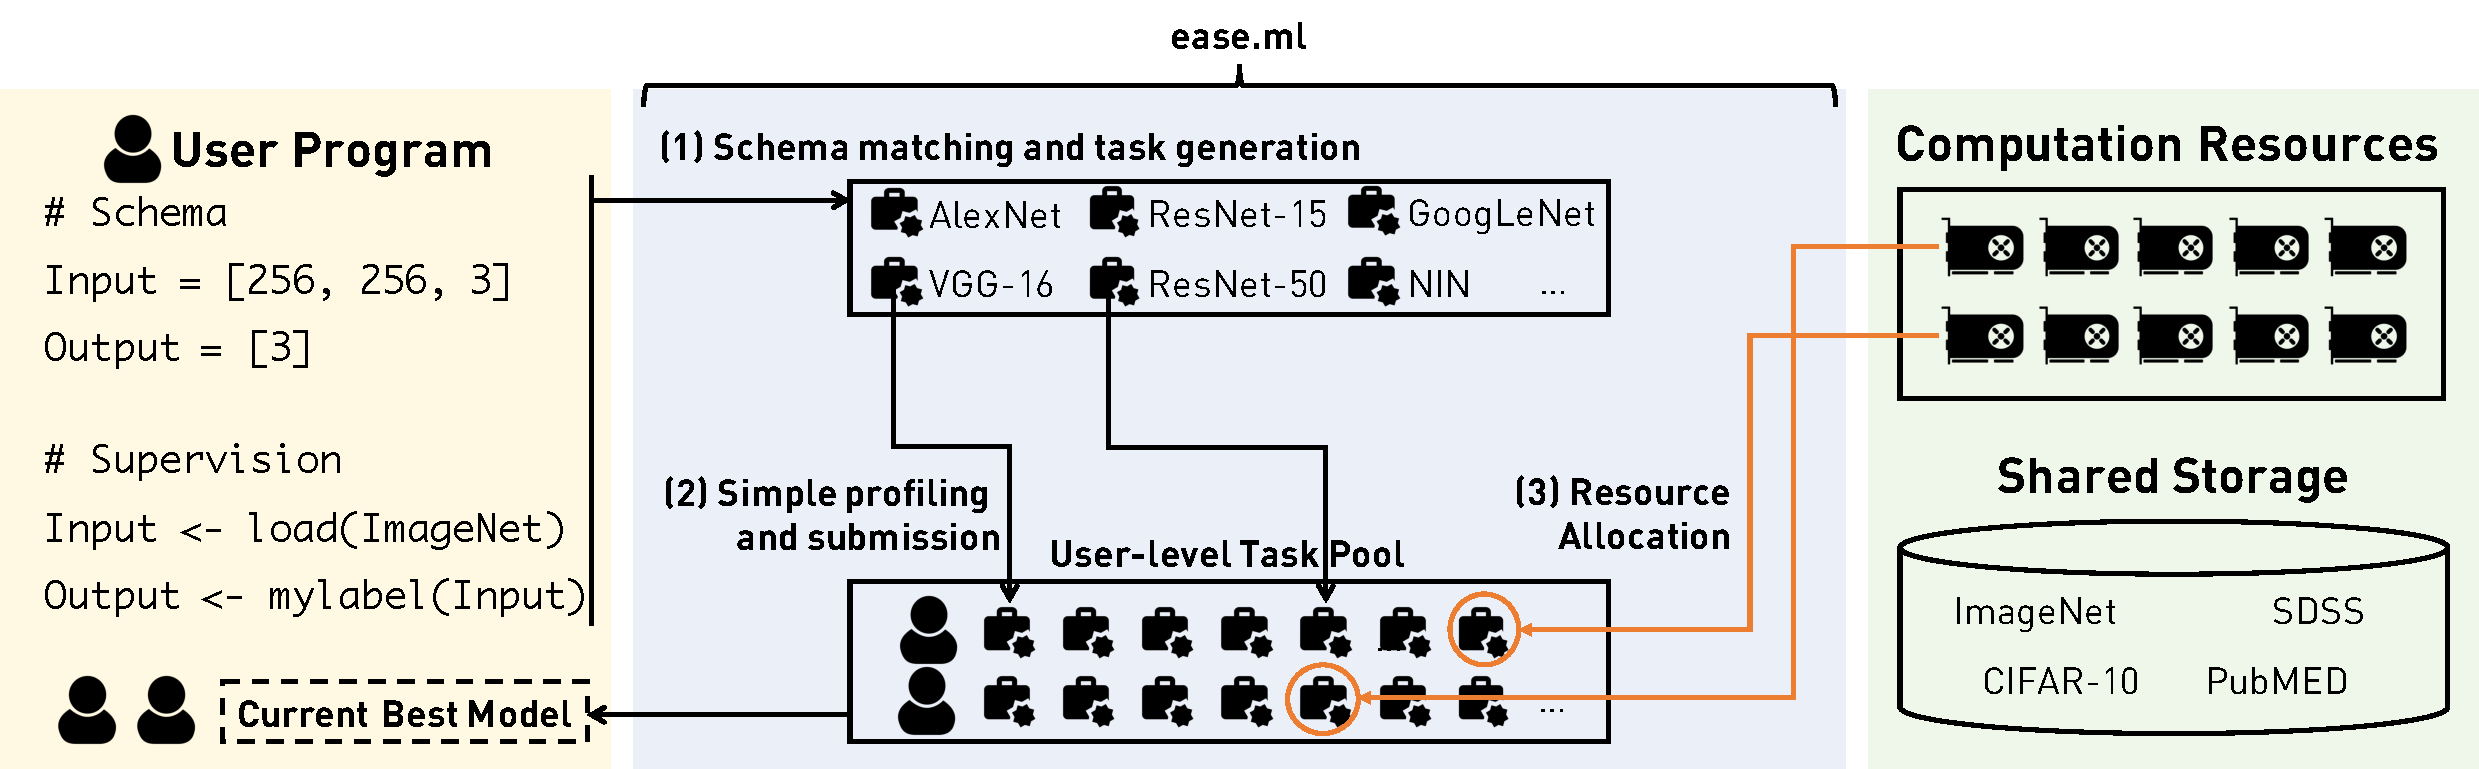
\includegraphics[width=0.8\textwidth]{figures/easeml}
\vspace{-1em}
\caption{System architecture of \texttt{ease.ml}.}
\label{fig:architecture}
\vspace{-1em}
\end{figure*}


\begin{figure}[t]
\centering
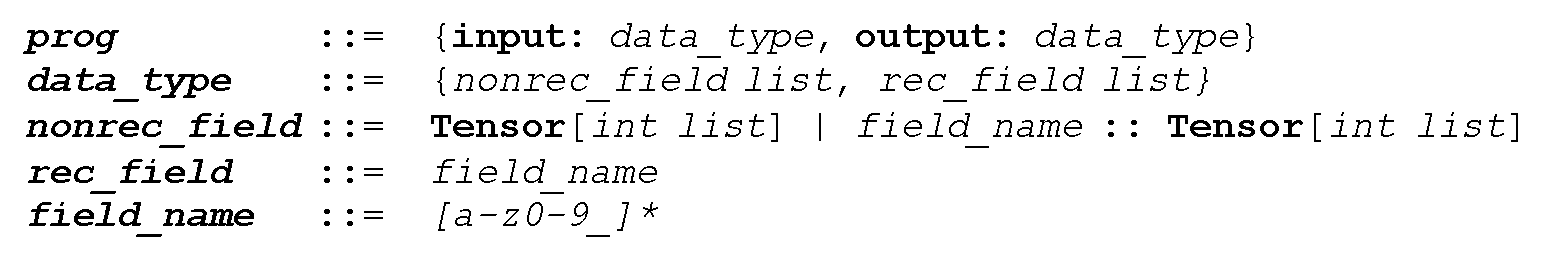
\includegraphics[width=0.5\textwidth]{figures/syntax}
\vspace{-2em}
\caption{Formal Syntax of an \eml Program}
\label{fig:syntax}
\vspace{-1em}
\end{figure}


%\section{Preliminaries}\label{sec:architecture}

%\subsection{System Architecture of ease.ml}
\vspace{-1em}
\section{System Architecture} \label{sec:architecture}

The design goal of \eml is two fold --- (1) provide an abstraction
to enable more effective model exploration for our users, and 
(2) manage the shared infrastructure to enable more efficient
resource utilization of the exploration process 
for {\em all}, instead of, {\em one} of our users.
The vision of \eml was published as a short vision paper
before~\cite{HILDA}, and this paper tackles the first
concrete technical problem we faced when realizing our
previous vision.

\eml provides a simple high-level, declarative language.
In \eml, user thinks about machine learning as an {\em arbitrary function approximator}.
To specify such an approximator, user provides the
system with (1) the size of the input, (2) the size of the output,
and (3) pairs of examples the function aims to approximate.
Figure~\ref{fig:architecture} illustrates the system architecture of \eml.

\vspace{-0.5em}
\subsection{System Architecture and Implementation}

We walkthrough each component of \eml and briefly
describe interesting design decisions
motivated by observing our users. 

\vspace{-1em}
\paragraph*{Input Program} The input
of \eml is a programming written in 
a simple domain specific language (DSL). Figure~\ref{fig:syntax}
shows the formal syntax of the DSL. To specify
a {\em machine learning task}, the user program (\textbf{\texttt{\em prog}})
contains the information about the {\em shape}
and {\em structure} of an input object (e.g., images, time series)
and an output object (e.g., class vector, images, time series).

The design goal of the structure of an input and output
object is to provide enough flexibility to support most
workloads we observed from our users. In the current design,
each object (\textbf{\texttt{\em data\_type}}) contains two parts:
(1) the ``recursive'' component (\textbf{\texttt{\em rec\_field}})
and (2) the ``non recursive'' component (\textbf{\texttt{\em nonrec\_field}}).
The recursive component contains a list of named 
field of the type of the same object, and the non recursive
component contains a list of constant-sized tensors.
This combination of recursive and non-recursive
components allows \eml to model a range of workloads
our users need, including image, time series, and trees.

\vspace{0.5em}
\noindent
{\bf (Example)} Figure~\ref{fig:walkthrough} shows
two example user programs for (1) image classification and (2) time series
prediction. For image classification, each input
object is a tensor of the size 256$\times$256$\times$3 and
each output object is a tensor of the size 1000 corresponding
to 1000 classes. Here both input
and output objects only contain the non-recursive component.
For time series prediction, each object not only
contains a 1-D tensor, but also contains
a ``pointer'' to another object of the same type. This
forms a time series. 


\begin{figure}[t]
\centering
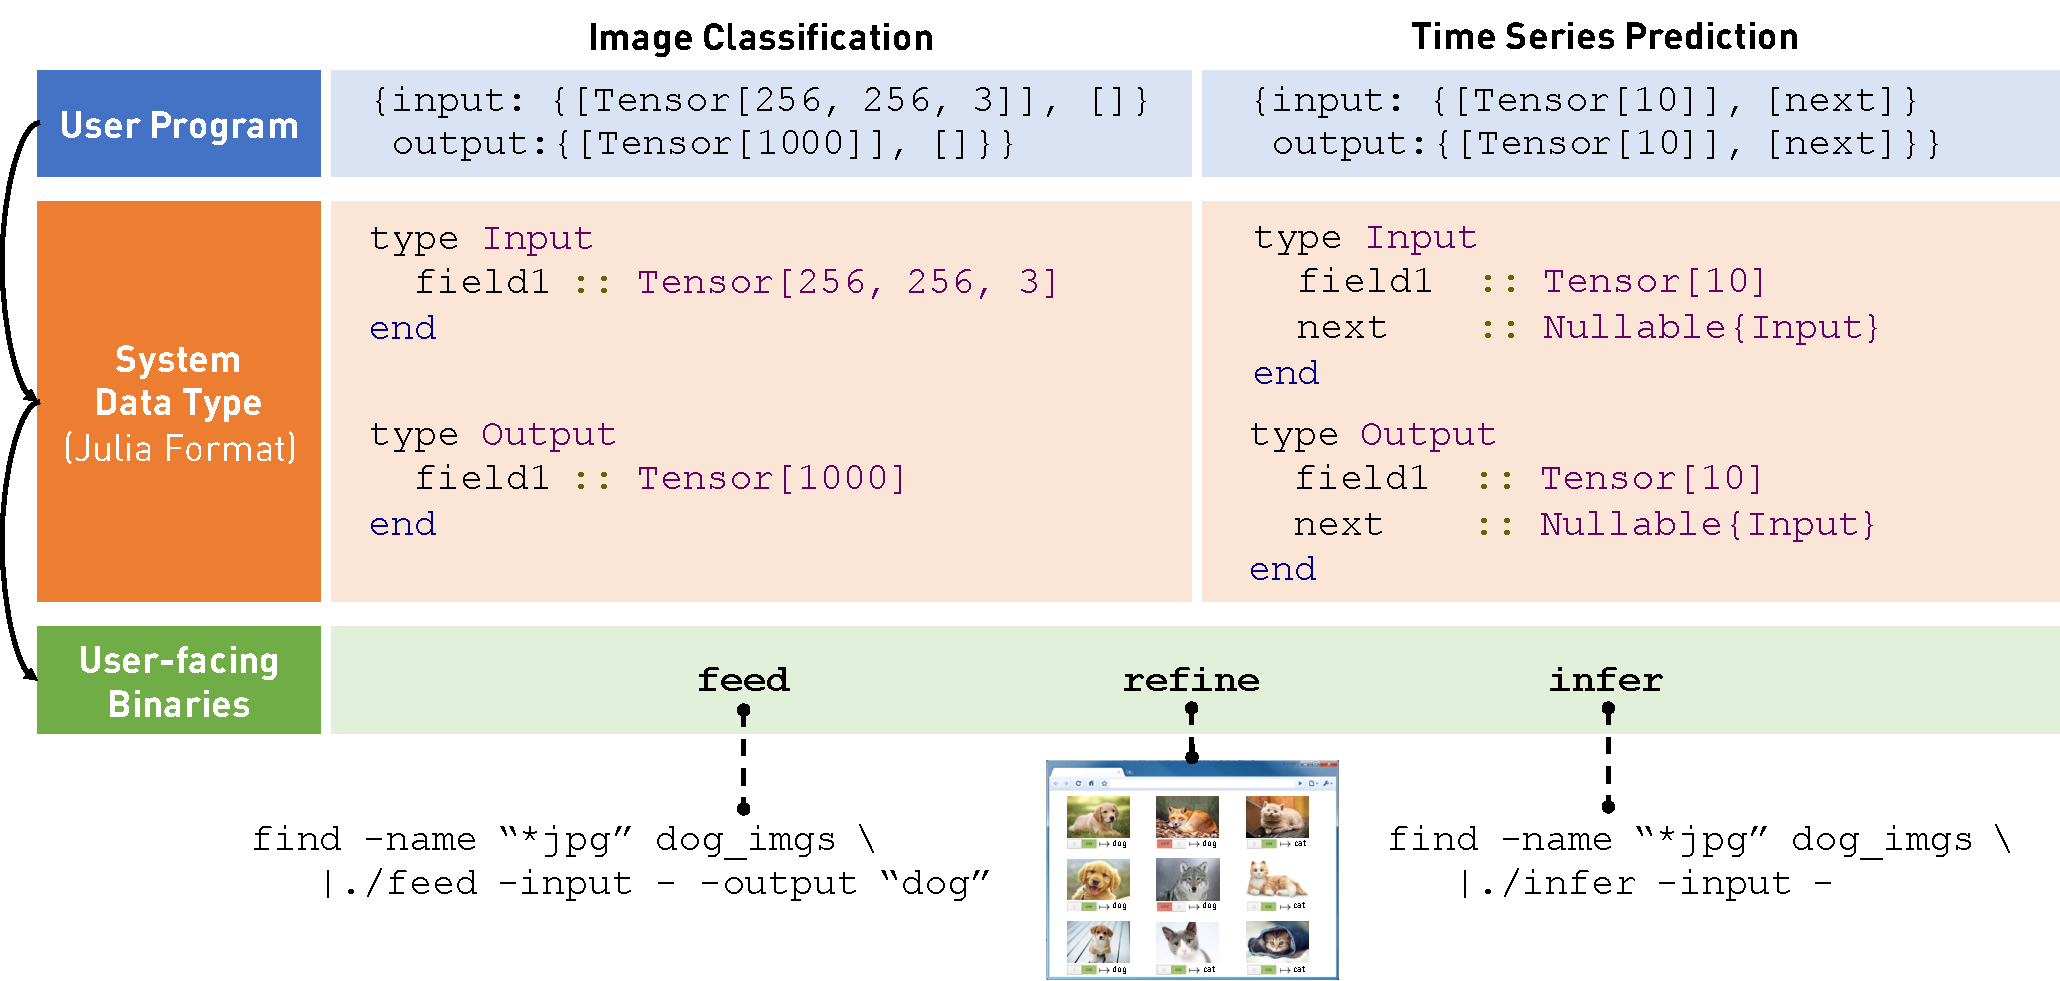
\includegraphics[width=0.5\textwidth]{figures/arch}
\vspace{-2em}
\caption{System Walkthrough}
\vspace{-2em}
\label{fig:walkthrough}
\end{figure}


\vspace{-2em}
\paragraph*{Code Generation and User Interaction}

Given an input program, \eml conducts code generation
to generate binaries that the user directly interacts with.
Figure~\ref{fig:walkthrough} illustrates the process.

In the first step of code generation, \eml translate
the user programs into {\em system data types}, data types
that the rest of the system is able to understand. 
Figure~\ref{fig:walkthrough} shows the system data types
generated in Julia. The translation process is based
on a very simple operational semantics and we omit the detail
here. One inherent assumption during the translation
is that there is no reuse of objects, i.e., we can 
only generate types corresponding to DAG without loop
(e.g., singleton, chains, and trees). 

Given the system data types generated by the translation
procedure, \eml then generates three binaries and
a Python library.
The Python library shares the same functionality as
the binaries but can be used in a programmable way.
Figure~\ref{fig:walkthrough} shows the three binaries
and Figure~\ref{fig:architecture} illustrates one
example in Python. The binaries and the Python library
contains a unique identifier and an IP address to the
\eml server. All operations the users conducted with
the generated binaries and Python library will be 
sent to the \eml server, which hosts the shared
storage and pool of computation resources.
There are three basic operations in \eml.

\noindent
{\textbf{1. \texttt{feed}}.} The \texttt{feed} operator takes
as input a set of input/output pairs. \eml provides
default loader for some popular Tensor types (e.g., loads
jpeg images into Tensor[A,B,3]). To associate an output
object and an input object, user can simply pipe a pair of
objects into the same as in Figure~\ref{fig:walkthrough}, or
write a {\em labeling function} that takes as input an input
object and generate an output object as shown in Figure~\ref{fig:architecture}.
Every time the user invokes the \texttt{feed} operator,
all data will be sent and stored in the centralized
\eml server.

\noindent
{\textbf{2. \texttt{refine}}.} The \texttt{refine} operator
shows all input/output pairs that the user ever \texttt{feed}'ed
into the system and allow the user to ``turn on''
and ``turn off'' each example. This is useful especially when
the users want to conduct data cleaning on the training set
to get rid of noisy labels introduced by weak/distant supervision.

\noindent
{\textbf{2. \texttt{infer}}.} The \texttt{infer} operator
takes as input an input object and output an output object
using the \textbf{{\em best model learned so far}}.

\paragraph*{Automatic Model Exploration}

The above interface provides user a high-level abstraction
in which the user only has a ``view'' of the best available model
instead of {\em what} model the system trains and 
{\em when} and {\em where} a model is trained. To enable 
this high-level interface, automatic model selection plays a
central role in \eml.

\vspace{0.5em}
\noindent
{\bf (Candidate Model Generation: Template Matching)} 
The first step of automatic
model exploration is to generate a set of 
candidate models given a user program. The current
version of \eml uses a template matching based approach.
Figure~\ref{fig:templates} shows the current set of
templates and the corresponding candidate models. 
The matching happens from the top to the bottom 
(from more specific template to more general template).

\vspace{0.5em}
\noindent
{\bf (Candidate Model Generation: Automatic Normalization)} 
Other than template matching, another source of candidate models 
comes from the automatic normalization feature 
in \eml. For image-shaped templates (e.g., Tensor[A,B,3]),
most consistent Deep Learning models are designed for
image data. However, many data from our users, although
has the shape like an image, have a much larger dynamic
range than an image. For one astrophysics application~\cite{MNRAS}
and one proteomics application, the dynamic range could
vary by more than ten orders of magnitude. In this case,
simply treating the input as an image results in unusable 
quality. \eml provides an automatic input/output
normalization feature by normalizing the input
with a family of functions as shown in Figure~\ref{fig:normalization}.
Each normalization function in this family, together with 
a consistent model, generates one additional 
candidate model.

\vspace{0.5em}
\noindent
{\bf (Automatic Model Selection)} 
Given a set of candidate models, \eml decides an order of
execution. The current execution strategy of \eml is to 
use {\em all} of its resources (29 GPUs) to train a single 
model in distributed CNTK. We made this design decision 
because we are able to achieve near-linear scale up
of training at this scale -- although in the near 
future \eml needs to allow more flexible resource 
allocation strategy to support a resource pool 
with hundreds of GPUs. Because there are different
users using \eml at the same time, \eml also needs
to decide which user to serve at the current time.
This motivates the technical problem of this paper
and we describe in details in Section~\ref{sec:multitenant}.

\paragraph*{Discussion: Hyperparameter Tuning}
We highlight one design decision in \eml
that is not optimal. \eml also conducts automatic
hyperparamter tuning but treats it as part of the
training procedure of a model -- for the model selection
subsystem, when it decides to train a given model,
it will always invoke a train procedure that conducts
automatic hyperparamter tuning. A more optimal design 
would be to fuse the hyperparamter tuning subsystem
with the model selection subsystem to better
utilize available resources to maximize the
{\em global happiness of all users}.






\begin{figure}[t]
\centering
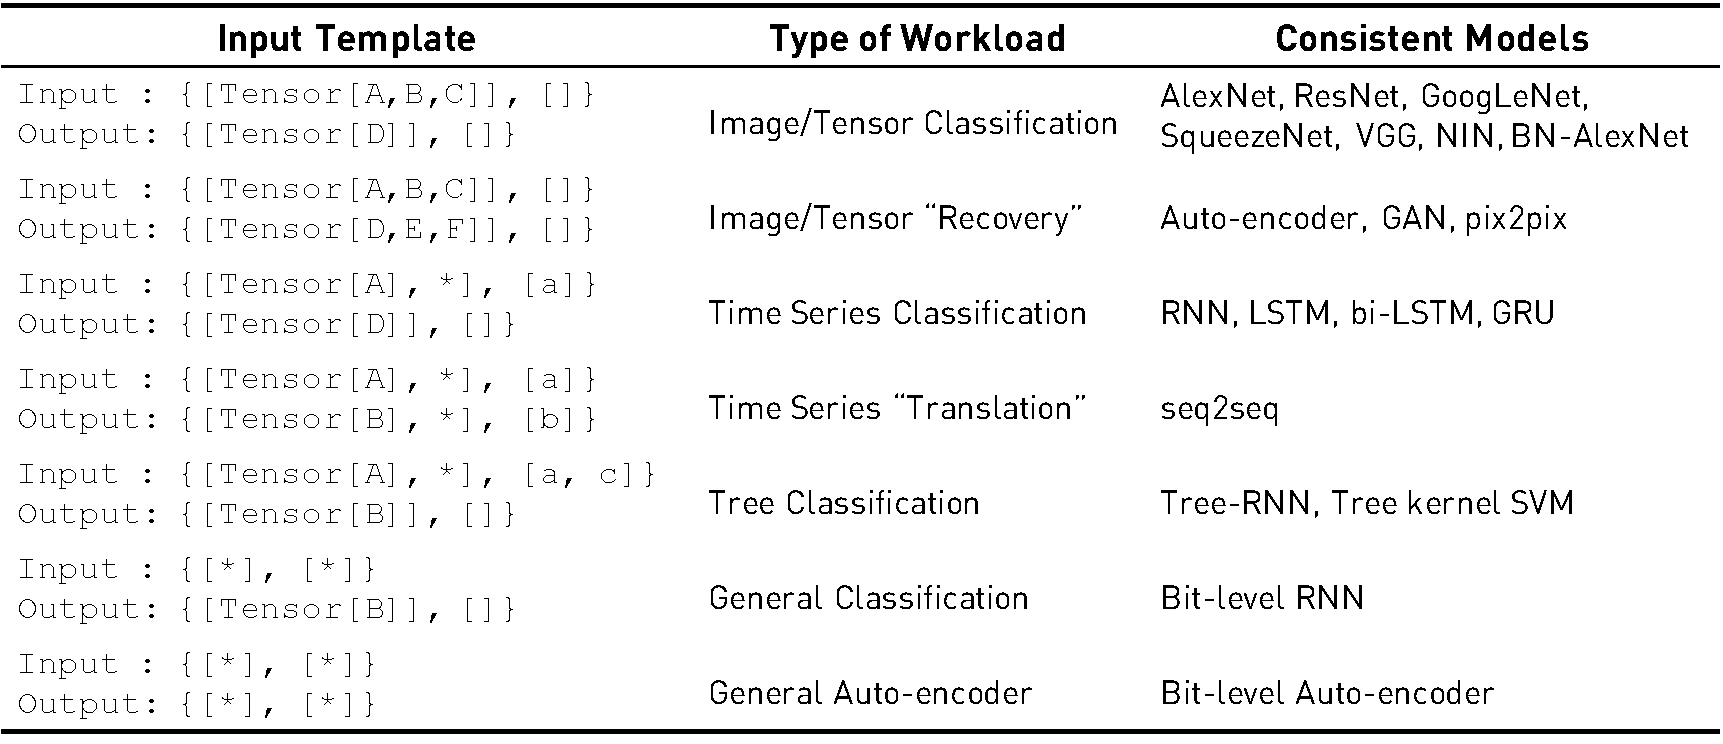
\includegraphics[width=0.45\textwidth]{figures/models}
\vspace{-1em}
\caption{Templates for candidate model generations. \texttt{A},
\texttt{B}, \texttt{C}, \texttt{D}, \texttt{E}, and \texttt{F}
are natural number constants; \texttt{a}, \texttt{b}, and \texttt{c} are of the type \texttt{\em field\_name}. \texttt{*} represents
matching for arbitrary ``tail'' of an array. Matching order
goes from top to bottom.}
\label{fig:templates}
\vspace{-1em}
\end{figure}

\begin{figure}[t]
\centering
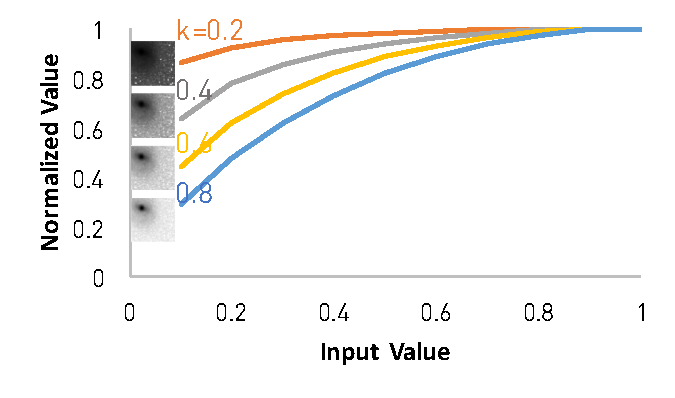
\includegraphics[width=0.3\textwidth]{figures/normalize}
\vspace{-2em}
\caption{Automatic normalization in \eml. Normalization function
is from $f_k(x) = -x^{2k} + x^{k}$ with different 
values of $k$. Each $k$ generates one additional candidate
model. Snapshots of a galaxy illustrate the impact of
normalization. Images from the astrophysics 
application~\cite{MNRAS} motivated this feature.}
 \label{fig:normalization}
\end{figure}


%\subsection{Single-tenant Model Selection}

%~
%\newpage
%%~
%\newpage


%\newpage
%~
%\newpage

\section{Multi-tenant Model Selection}\label{sec:multitenant}

Although the single-tenant model selection problem has been extensively studied in the literature, the multi-tenant model selection problem is new as far as we know.
It should not be a sheer surprise, as multi-tenancy only comes into the picture when machine learning is offered as a service that is hosted by a shared infrastructure, which did not happen until quite recently.

In this section, we give a first formulation to the problem and propose a solution to it.
Our problem formulation is an extension to the classic view of model selection as a bandit problem.
Basically, we extend the bandit problem from the standard single-tenant, cost-oblivious (STCO) setting to the multi-tenant, cost-aware (MTCA) setting.
Our solution is then based on extending the well-known STCO GP-UCB algorithm, a technique that combines the UCB (shorthand for ``upper confidence bound'') heuristic with Bayesian optimization, with the goal of minimizing the total regret of all users.
We further present a detailed theoretical analysis and show that our solution can achieve a regret bound in line with the best ones known for the STCO GP-UCB algorithm.

\subsection{Preliminaries}

Model selection can be viewed as a multi-armed bandit problem.
Each algorithm corresponds to an \emph{arm} of the bandit, whereas the observed evaluation result of the algorithm corresponds to the \emph{reward} of playing the conceivable arm.
A common optimization criterion is to minimize the average \emph{regret} as time goes by.

Formally, let $x_t$ be the reward of playing some arm $k\in[K]$ at time $t$, and let $x_{*,t}=\max\{x_{k,t}\}$ where $k\in[K]$.
The {\em instantaneous} regret at time $t$ is then
\begin{equation}\label{eq:instant-regret}
r_t=x_{*,t}-x_t,
\end{equation}
whereas the {\em cumulative} regret up to time $T$ is defined as 
\begin{equation}\label{eq:cumulative-regret}
R_{T}=\sum\nolimits_{t=1}^{T}r_t.
\end{equation}
A desired property of a solution to the bandit problem is
\begin{equation}\label{eq:regret-free}
\lim\nolimits_{T\to\infty}R_T/T=0,
\end{equation}
namely, asymptotically there is no cumulative regret.

\subsection{Problem Formulation}

Suppose that we have $K$ candidate models/algorithms hosted by a shared machine learning infrastructure.\footnote{We will use ``models'' and ``algorithms'' exchangeably.}
Consider a multi-tenant scenario where we have $n$ users and each user $i\in[n]$ has his/her own machine learning task represented by a dataset $D_i$.
For a dataset $D$ (from a user), we use $\cA_k(D) \in \R$ to denote the performance (e.g., prediction accuracy) of $\cA_k$ on $D$ and $\cA(D) \in \R^K$ to denote the performance of all algorithms on $D$.
The goal is to find out the best algorithm for $D$ with cost as low as possible.
For simplicity, we assume that the outcome of applying an algorithm to $D$ is deterministic.
Here, the cost of $D$ is defined as the overhead (e.g., time) of evaluating the algorithm ``once'' on $D$.
For example, in the case of model section via hyper-parameter tuning, one evaluation could be trying one specific hyper-parameter combination within the whole search space.
In the context selecting deep neural networks, one evaluation could be running one iteration of training under a given hyper-parameter setting.
We can further introduce the notion of \emph{prior distribution} regarding the performance of each algorithm based on historical executions.
Figure~\ref{fig:problem-formulation} presents a canonical view of the problem formulation in this general setting where (partial) knowledge about model performance is available.

\begin{figure}[t]
\centering
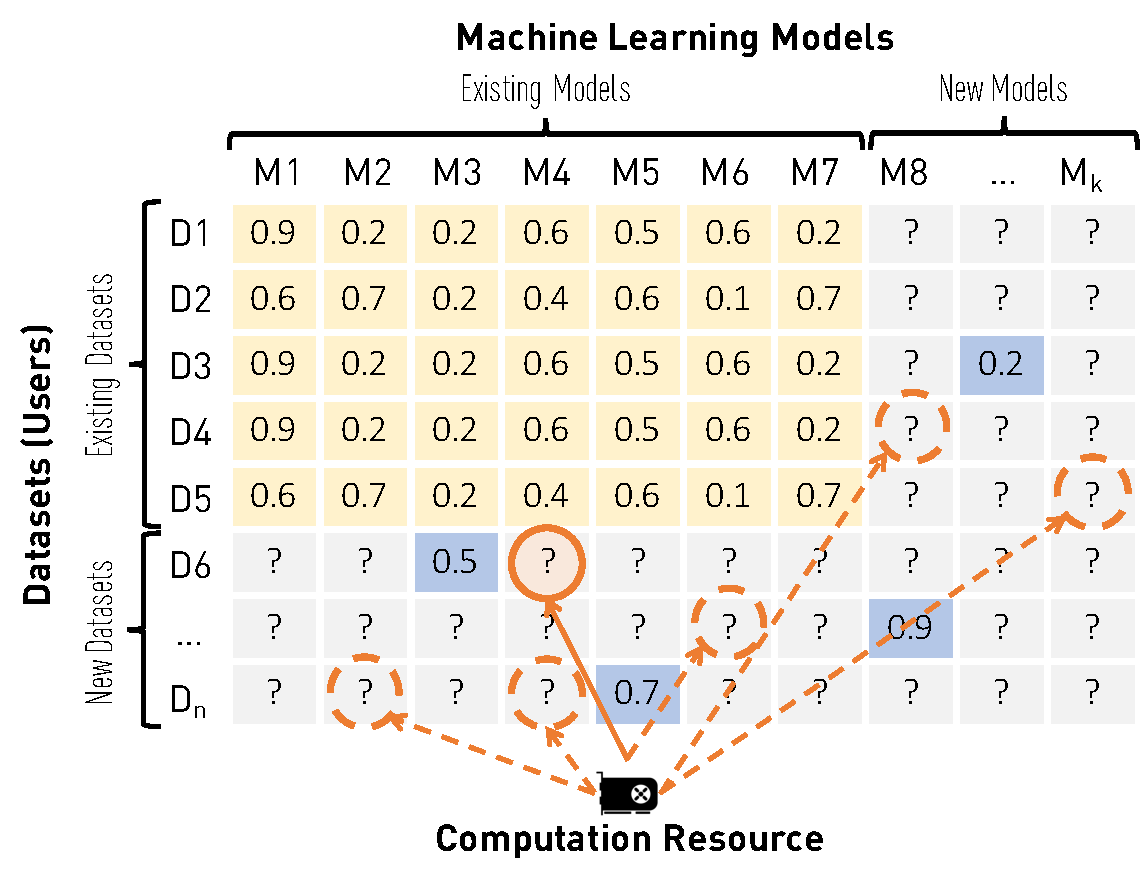
\includegraphics[width=0.9\columnwidth]{figures/multitenant}
\vspace{-2em}
\caption{A canonical view of the multi-tenant, cost-aware model selection problem we studied in this paper.}
\label{fig:problem-formulation}
\vskip -2ex
\end{figure}

\textbf{Extended Semantics for Regrets:} When moving to the MTCA setting, the definitions of instantaneous and cumulative regrets need to be extended.
Given that only one user is scheduled at any time step $t$, how should we define the instantaneous regret for a user that is not scheduled at $t$?
Note that the $r_t$ in Equation~\ref{eq:instant-regret} is not defined for unscheduled user.
This would be difficult if negative rewards were allowed.
Fortunately, we have restricted reward in model selection as the observed model performance, which must be positive.
As a result, we can simply set $x_t=0$ in Equation~\ref{eq:instant-regret} for a user that is not scheduled at $t$, namely, the user incurs the maximum regret for being ignored.
The definition for cumulative regret (Equation~\ref{eq:cumulative-regret}) remains the same under this extended semantic.

The remaining question is the optimization goal.
A solution to the STCO bandit problem aims for minimizing the time-averaging regret $R_T/T$ for a given time $T$, which goes to zero as $T$ goes to infinity if the solution is regret-free (Equation~\ref{eq:regret-free}).
A natural extension could be then to minimize the time-averaging regret for each user (at the same given time $T$) simultaneously.
However, this is apparently unfeasible even if all users are homogeneous (i.e., they provide the same models running on the same datasets), because reducing the regret of one user will unavoidably increase the regrets of the others.
This implies that absolute fairness is not achievable in multi-tenancy: We have to sacrifice fairness for better efficiency.
Here we propose to minimize the total regret of all users, which is another natural extension to the STCO case.
Formally, let $R_T^i$ be the cumulative regret (under the extended semantics of regrets) of user $i\in[n]$ at time $T$.
We aim for minimizing
\begin{equation}\label{eq:time-avg-regret}
R_T/T=\frac{1}{T}\sum\nolimits_{i=1}^n R_T^i.
\end{equation}
The regret-free property remains desirable.

\newpage

\subsection{Cost-aware Single-tenant GP-UCB}

We start by presenting the standard GP-UCB algorithm that targets the STCO bandit problem.
Essentially it is a combination of using the upper confidence bound (UCB) heuristic and the Gaussian process (GP), a Bayesian optimization approach to nonlinear regression.
The UCB heuristic prefers the arm that maximizes the quantity $\mu_k + \theta\cdot\sigma_k$, where $\mu_k$ and $\sigma_k^2$ are the observed mean and variance of the reward distribution of the arm $k\in[K]$.
This is essentially just the upper bound of the $\theta$-confidence interval (and thus the reason for the name UCB).
Despite its simplicity, it exhibits a good trade-off between \emph{exploration} and \emph{exploitation}.
Intuitively, the UCB heuristic favors arms with high reward (for exploitation), \emph{and} high uncertainty (for exploration), which implies high risk but also high opportunity for gaining better reward.
The GP-UCB algorithm further leverages GP to guide the search space from which the target reward function should be sampled.
As more and more arms are attempted, the GP-UCB algorithm can quickly converge to identification of the best arm (i.e., best model in the context of model selection).
Algorithm~\ref{alg:gp-ucb} presents the details of GP-UCB.

\begin{algorithm}[t]    
\scriptsize
\caption{Single-tenant, cost-oblivious GP-UCB}          % give the algorithm a caption
\label{alg:gp-ucb}                           % and a label for \ref{} commands later in the document
\begin{algorithmic}[1]                    % enter the algorithmic environment
   \REQUIRE GP prior $\mu_0$, $\sigma$, $\Sigma$, and $\delta\in (0,1)$
   \ENSURE Return the best algorithm among all algorithms in $a_{[1:T]}$
   \STATE Initialize $\sigma_0 = \text{diag}(\Sigma)$
   \FOR {$t=1,2,\cdots, T$}
   \STATE $\beta_t \rightarrow \log (Kt^2/\delta)$\\
   \STATE $a_t \rightarrow \argmax_{k\in [K]}\mu_{t-1}(k) + \sqrt{\beta_t}\sigma_{t-1}(k)$\\
   \STATE Observe $y_t = \cA_{a_t} + \epsilon_t$\\
   \STATE $\mu_t(k) = \Sigma_t(k)^\top (\Sigma_t + \sigma^2 I)^{-1} y_{[1:t]}$\\
   \STATE $\sigma_t^2(k) = \Sigma(k, k) - \Sigma_t(k)^\top(\Sigma_t + \sigma^2 I)^{-1} \Sigma_t(k)$
   %\STATE $\cA_K = \text{arg}\max_{k \in [K]} \mu_t(k) + \sqrt{\beta_t} \sigma_{t}(k)$
   \ENDFOR
\end{algorithmic}
%\hline
\vspace{0.5em}
\textbf{Notation}:
\begin{itemize}
\item $[K] = \{1, 2, \cdots, K\}$.
\item $a_{[1:t]} = \{a_1, \cdots, a_t\}$, where $a_i \in [K],$ for $1\le
  i\le t$.
\item $y_{[1:t]} = \{y_1, \cdots, y_t\}$.
\item $\Sigma(i,j) = \Sigma_{i,j}$, for $i,j\in [K]$.
\item $\Sigma_t(k) = [\Sigma(a_1, k), \cdots \Sigma(a_t,k)]^\top, k\in [K]$.
\item $\Sigma_t = [\Sigma(i, j)]_{i,j\in a_{[1:t]}}$.
\item $\epsilon_t \sim \mathcal{N}(0, \sigma^2)$.
\end{itemize}
\end{algorithm}


\begin{figure}
\centering
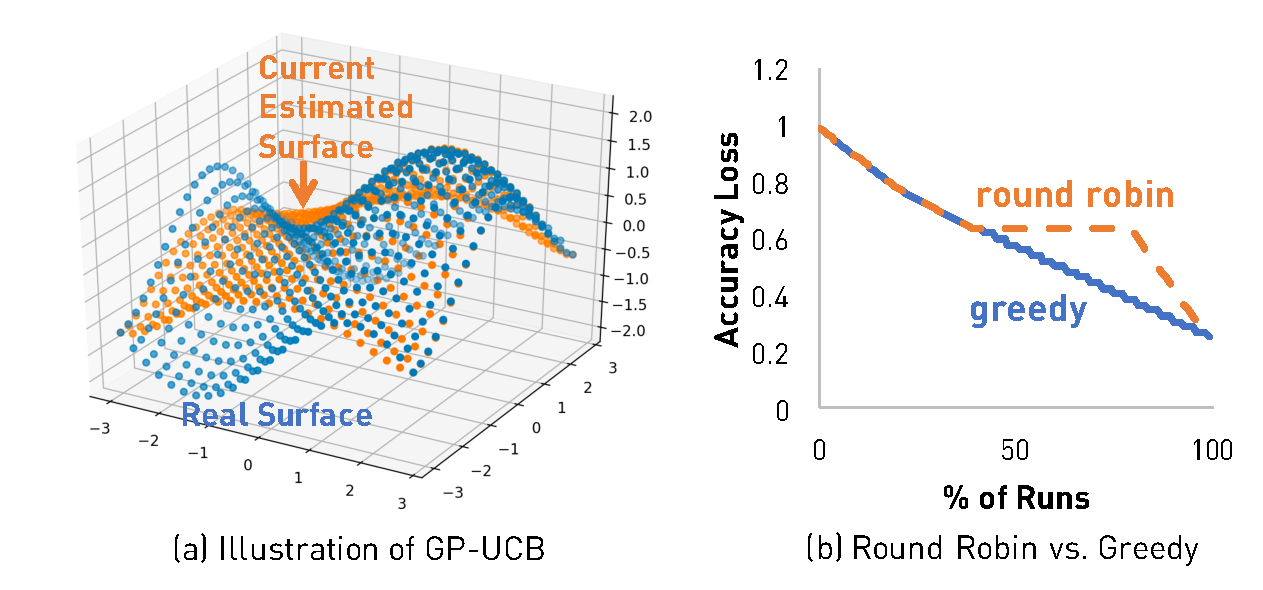
\includegraphics[width=0.45\textwidth]{figures/rr_v_greedy}
\vspace{-1em}
\caption{Illustration of the difference between \textsc{RoundRobin}
and \textsc{Greedy} in multi-tenant setting.}
\label{fig:gpucb-intuition}
\vskip -2ex
\end{figure}


We highlight the selection rule (i.e., the {\em allocation policy} in the bandit literature) in Algorithm~\ref{alg:gp-ucb} below, which is a slight variant of the aforementioned UCB heuristic:
\begin{equation}\label{eq:gp-ucb}
a_t = \argmax_{k\in [K]}\{\mu_{t-1}(k) + \sqrt{\beta_t}\sigma_{t-1}(k)\}.
\end{equation}
The $\beta_t$ in Equation~\ref{eq:gp-ucb} is a parameter that controls the convergence rate. With the choice of $\beta_t$ as was shown in Algorithm~\ref{alg:gp-ucb}, the regret $R_T$ can be bounded as $O(\sqrt{T})$ (up to polylog factors) with high probability. Therefore, GP-UCB is regret-free.

The GP-UCB algorithm, as well as other solutions to the bandit problem, does not consider the cost of a trial.
The arms are treated as homogeneous and the (potentially huge) cost difference in playing different arms is completely ignored.
Apparently, more sophisticated machine learning models usually incur higher training overhead so it makes sense in practice to further consider the cost when selecting a model for evaluation.
In a multi-tenant context, different users usually vary dramatically in their cost budgets.
Ignoring the cost respect may therefore end up with selecting poor models for budget-stringent users, due to running out of budget and premature stop in model evaluation.
Moreover, the performance of different models may correlate quite differently for different users, depending on the properties of the datasets, which further complicates the model selection problem.

Therefore, we next extend the standard GP-UCB algorithm to a cost-aware version.
We restrict ourselves in the single-user case but introduce the notion of cost into Algorithm~\ref{alg:gp-ucb}.
The idea is simple. We basically replace Equation~\ref{eq:gp-ucb} by the following:
\begin{equation}\label{eq:gp-ucb:cost}
a_t = \argmax_{k\in [K]}\{\mu_{t-1}(k) + \sqrt{\frac{\beta_t}{c_k}}\sigma_{t-1}(k)\}.
\end{equation}
Here $c_k$ is the cost for one evaluation of the model $k\in[K]$.
Intuitively, this implies that we need to lower priority for expensive models even if they have high observed reward and uncertainty.

\paragraph*{Theortical Analysis}

{\color{red} Single tenant, cost-aware case}

% Given $\delta\in (0,1)$ and a sequence of positive numbers $\{c_k\}_{k=1}^K$,
% consider the following optimization problem
% \begin{equation}
%   \label{eq:beta}
%   \text{minimize}\quad \max_{t\in [T]}~\beta_t,
% \end{equation}
% subject to
% \[
%   \sum_{t=1}^T\sum_{k = 1}^K e^{-\frac{\beta_t}{2c_k}}\le \delta.
% \]

\begin{theorem}
  \label{thm:cost}
  Given $\delta\in (0,1)$ and set $\beta_t = 2c^\ast \log\left[\frac{\pi^2 K t^}{6\delta}\right]$ with $c^\ast = \max_{k\in [K]}\{c_k\}$.
  Then the
  simple regret of the single tenant, cost-aware GP-UCB is bounded above by
  $\sqrt{I(T)/(\sum_{t=1}^Tc_{a_t})}$ with probability at
  least $1-\delta$, i.e.,
  \[
    \bP\left(\min_{t\in [T]}r_t \le \sqrt{\frac{I(T)}{\sum_{t=1}^T
        c_{a_t}}}\right) \ge 1-\delta,
\]
where 
\[
I(T) = \frac{4\beta_T}{\log(1 + \sigma^{-2})}\sum_{t=1}^T \log(1+\sigma^{-2}\sigma^2_{t-1}(a_t))
\]
\end{theorem}



\newpage

\begin{algorithm} [t]                     % enter the algorithm environment
\scriptsize
\caption{Multi-tenant GP-UCB}          % give the algorithm a caption
\label{alg:mc-general}                           % and a label for \ref{} commands later in the document
\begin{algorithmic}[1]                    % enter the algorithmic environment
   \REQUIRE GP prior $\{\mu_0^i\}_{i=1}^n$, $\{\sigma^i\}_{i=1}^n$, $\{\Sigma^i\}_{i=1}^n$, and $\delta\in (0,1)$
   \ENSURE Return the best algorithm among all algorithms in $a_{[1:T]}^i$ for all users $i=1, \cdots, n$.
   \FOR{$i=1,...n$}
       \STATE Initialize $\sigma_0^i = \text{diag}(\Sigma^i)$ and $t_i=1$
       \STATE Run one step of GP-UCB (i.e., lines 3 to 5 of Algorithm~\ref{alg:gp-ucb}) for the user $i$ to obtain $\sigma^i_{t_i}$ and $\mu^i_{t_i}$
   \ENDFOR
   %\STATE Initialize $\sigma_0^i = \text{diag}(\Sigma^i)$ and $t_i=1$
   %\STATE Run GP-UCB for all users once and obtain $\sigma^i_{t_i}$, $\mu^i_{t_i}$
   \FOR {$t=1,...,T$}
        \STATE Refine regrets for users $i\in[n]$ with new observations
        \[
   %\tilde{\sigma}^i_{t_i-1} = \underbrace{\min\left\{B_{t_i-1}(a^i_{t_i-1}), \min_{t'<t_i-1} y^i_{t'}+ \tilde{\sigma}^{i}_{t'} \right\}}_{\text{Estimate the $f^*$}} - y^i_{t_i-1}
   \tilde{\sigma}^i_{t_i-1} = \min\left\{B_{t_i-1}(a^i_{t_i-1}), \min_{t'<t_i-1} y^i_{t'}+ \tilde{\sigma}^{i}_{t'} \right\} - y^i_{t_i-1} 
   \]
      \STATE Decide the candidate set
   \[
     V_t := \left\{ i\in [n]: 
         \tilde{\sigma}^i_{t_i-1} \ge \frac{1}{n}
       \sum_{i=1}^n 
         \tilde{\sigma}^i_{t_i-1}\right\}
   \]
   \STATE Select a user (using any rule) from $V_t$ indexed by $j$

   \STATE  Update $\beta_{t_j}^j$ by
   \[
     %\beta_{t_i}^i = \text{\color{red}constant} \times \log (K^it_{\color{red}i}^2/\delta)
     \beta_{t_j}^j = \log (K^j t_j^2/\delta)
   \]
   \STATE Select the best algorithm for the user $j$
   \[
     a^j_{t_j} = \argmax_{k\in [K^j]}\mu^j_{{t_j}-1}(k) + \sqrt{\beta^j_{t_j}}\sigma^j_{t_j-1}(k)
     \]
     \STATE Observe $y^j_{t_j}(a^j_{t_j})$

     \STATE Update $\sigma^j_{t_j}$ and $\mu^j_{t_j}$ (see lines 4 and 5 in Algorithm~\ref{alg:gp-ucb})
        \STATE Increase the count of the user $j$ by $t_j \leftarrow t_j + 1$
   \ENDFOR
\end{algorithmic}
\end{algorithm}


\subsection{Multi-tenant GP-UCB}

\subsubsection{Round Robin GP-UCB}



\paragraph*{Theoretical Analysis}

{\color{red} Round Robin, cost-aware case}

\begin{theorem}
  \label{thm:rr}
  Given $\delta\in (0,1)$ and set $\beta_t^i = 2c^\ast \log\left[\frac{\pi^2 n K^\ast t^2}{6\delta}\right]$ with $c^\ast = \max_{i\in [n], k\in [K^i]}\{c^i_k\}$ and $K^\ast = \max_{i\in [n]}\{K^i\}$. Then the
  total regret of Round Robin GP-UCB is bounded above by
  \[
     \sqrt{n T}\sum_{i=1}^n \sqrt{I([T(i)])}
  \]
  with probability at least $1-\delta$,
  where
  \begin{align*}
    I([T(i)]) & = 4 \sqrt{\frac{c^\ast \beta^\ast}{\log(1 + (\sigma^\ast)^{-2})}}\\
    &\qquad \sum_{t\in T(i)} \log\left(1 + (\sigma^i)^{-2}(\sigma^i_{t-1}(a^i_{t}))^2\right),
  \end{align*}
  with $\sigma^\ast= \max_{i\in [n]}\{\sigma^i\}$ and $\beta^\ast = 2c^\ast \log\left[\frac{\pi^2 n K^\ast T^2}{6\delta}\right]$.
\end{theorem}



\newpage

\subsubsection{Multi-tenant GP-UCB}

We now extend the single-tenant, cost-aware GP-UCB algorithm to the multi-tenant case.
For ease of exposition, we define $B_t(k)$ to be the upper confidence bound of the model $k\in[K]$ at the time $t$: %namely,
\begin{equation}
B_t(k)=\mu_{t-1}(k) + \sqrt{\beta_t}\sigma_{t-1}(k).
\end{equation}
Under this notation, for example, Equation~\ref{eq:gp-ucb} can be simplified as $a_t=\argmax_{k\in [K]} B_t(k)$.

%\begin{equation}
%\sqrt{\beta_{t_i-1}}\sigma_{t_i-2}(a^i_{t_i-1}) + \mu_{t_i-2}(a^i_{t_i-1}).
%\end{equation}

Algorithm~\ref{alg:mc-general} presents the details of the multi-tenant GP-UCB algorithm.
(We only present the cost-oblivious version of the algorithm --- the cost-aware version is simply replacing all occurrences of $\sqrt{\beta}$ by $\sqrt{\beta/c}$, where $c$ is the corresponding cost.)
It consists of two phases.
In the first phase (lines 6 to 8), we determine which user to schedule next (i.e., the \emph{user selection} phase).
In the second phase (lines 9 to 12), we determine which model to run for this user (i.e., the \emph{model selection} phase).
The model selection phase is straightforward --- we choose the model with respect to the single-tenant GP-UCB criterion. (Compare lines 9 to 12 in Algorithm~\ref{alg:mc-general} with lines 3 to 5 in Algorithm~\ref{alg:gp-ucb}.)
The user selection phase is more sophisticated as we shall discuss next.



One idea for user selection is to compare the best models (based on Equation~\ref{eq:gp-ucb}) from different users and pick ``the best of the best.''
However, in what sense are the best models comparable?
To understand the subtlety here, consider two models $M_1$ and $M_2$ from two users.
Suppose that, at a certain time step $t$, the mean accuracy of $M_1$ and $M_2$ are 0.9 and 0.7, respectively.
Moreover, assume that the Gaussian variances of $M_1$ and $M_2$ are the same.
The UCB criterion (Equation~\ref{eq:gp-ucb}) will then favor $M_1$ over $M_2$.
In the single-tenant case this makes perfect sense: $M_1$ is a clear win over $M_2$.
In the multi-tenant case this is perhaps indefinite, because it is possible that $M_1$ is working on an easy dataset whereas $M_2$ is working on a hard one.
Therefore, the mean accuracy in the UCB criterion (i.e., the $\mu$ part in Equation~\ref{eq:gp-ucb}) is not a reliable indicator of the potential model improvement when comparing different users.
Based on this observation, we choose to omit the mean accuracy in the UCB criterion and focus on the observed variance.

This leads to the specific user selection strategy illustrated in lines 6 to 8 of Algorithm~\ref{alg:mc-general}.
In line 6, we first compute more accurate regrets for users with new observations.
In fact, except for the initialization stage (lines 1 to 4) where more than one user has new observation, there is only one user with new observation at each subsequent time step, as we only schedule one user at a time.
We define $\tilde{\sigma}_t^i$ to be the \emph{empirical variance} observed for the user $i$ at the time $t$, and define 
\begin{equation}\label{eq:emp-bound}
b_t^i=y_t^i + \tilde{\sigma}_t^i
\end{equation}
to be the \emph{empirical confidence bound} (to distinguish it with the upper confidence bound).
Using the above notation, the refinement formula in line 6 can then be rewritten as
\begin{equation}\label{eq:emp-bound-recurrence}
b_{t_i-1}^i=\min\left\{B_{t_i-1}(a^i_{t_i-1}), \min_{t'<t_i-1} b^i_{t'}\right\}.
\end{equation}
Clearly, Equation~\ref{eq:emp-bound-recurrence} represents a recurrence relation on the empirical confidence bounds.
Assuming that the user $i$ was scheduled at the time $t-1$, the empirical confidence bound for the user $i$ after the time $t-1$ (i.e., at the time $t$) is either the updated upper confidence bound $B_{t-1}$
or the minimum empirical confidence bound before the time $t$, whichever is smaller (i.e., tighter).
Intuitively, the empirical confidence bound tries to tighten the upper confidence bound by utilizing the observed reward more directly: The upper confidence bound criterion merely uses the observations to update the parameters of the Gaussian process, which may result in slower convergence (or equivalently, larger/looser bound) if the observations are distant from the Gaussian priors.
By Equation~\ref{eq:emp-bound}, the empirical variance is then computed by subtracting the observed reward from the empirical confidence bound.

In lines 7 and 8, we further use the empirical variances of the users to determine which one to schedule next.
(As we have noted above, variances, but not means, matter when contrasting different users.)
Specifically, we first decide a set of candidate users whose empirical confidence bounds are above the average, and then pick one user from the candidates.
The criterion we use to choose the candidates is based on somewhat technical reasons: We want to bound the regret rate of Algorithm~\ref{alg:mc-general}.
This will become clear in our theoretical study, though the intuition is not difficult to explain.
{\color{red}
By choosing a user with confidence bound above the average, we can reduce the time-averaging regret defined in Equation~\ref{eq:time-avg-regret}.
It is interesting that the regret bound remains the same regardless of the rule for picking a user from the candidates, though in practice different rules may make a difference.
For example, picking the user with the maximum empirical variance may be better than randomly picking a user.
In our experiments, we pick the user with the maximum \emph{expected improvement} from the candidates, which shows good performance.
Nevertheless, the existence of an optimal strategy in the practical sense remains as an open question.
}

One might wonder if we can just replace the empirical variance by the Gaussian variance as in the UCB criterion (i.e., replace $\tilde{\sigma}$ by $\sigma$).
{\color{red} Theoretically, the answer is yes and we can obtain similar regret bound.}
However, as we have pointed out, in practice using the empirical variance can give much better performance --- the empirical confidence bound by directly leveraging the observation can be much tighter compared with the upper confidence bound.
A more surprising fact here is that, if we only care about the theoretical regret bound, then the user selection phase is unimportant --- using a round-robin strategy will give the same regret bound!
We next discuss this by-product in more detail by presenting a theoretical analysis of Algorithm~\ref{alg:mc-general}.

\paragraph*{Theoretical Analysis}

{\color{red} Multi-tenant, cost-aware case}

% Given $\delta\in (0,1)$ and a sequence of positive numbers $\{c_k^i\}$,
% consider the following optimization problem
% \begin{equation}
%   \label{eq:beta-multi}
%   \text{minimize}\quad \max_{t\in [T]}~\beta^i_t,
% \end{equation}
% subject to
% \[
%   \sum_{t=1}^T\sum_{i=1}^n\sum_{k = 1}^{K^i} e^{-\frac{\beta^i_t}{2c^i_k}}\le \delta.
% \]

\begin{theorem}
  \label{thm:multi-cost}
  Given $\delta\in (0,1)$ and set $\beta_t^i = 2c^\ast \log\left[\frac{\pi^2 n K^\ast t^}{6\delta}\right]$ with $c^\ast = \max_{i\in [n], k\in [K^i]}\{c^i_k\}$ and $K^\ast = \max_{i\in [n]}\{K^i\}$. Then the
  total regret of Multi-tenant GP-UCB is bounded above by
  \[
    n \sqrt{T}\sqrt{\sum_{i=1}^n I([T(i)])}
  \]
  with probability at least $1-\delta$,
  where
  \begin{align*}
    I([T(i)]) & = 2 \sqrt{\frac{c^\ast \beta_T}{\log(1 + (\sigma^\ast)^{-2})}}\\
    &\qquad \sum_{t\in T(i)} \log\left(1 + (\sigma^i)^{-2}(\sigma^i_{t-1}(a^i_{t}))^2\right),
  \end{align*}
  with $\sigma^\ast= \max_{i\in [n]}\{\sigma^i\}$.
\end{theorem}

It is observed that $I([T(i)])$ is proportional to the information gain for each user $i$. In particular, if the kernel function or covariance matrix is linear (see
  Theorem 5 in \cite{srinivas2009gaussian}), then for each $i\in [n]$, the
  order of $I([T(i)])$ is at most $\log(|T(i)|)$. Since
  \[
    \sum_{i=1}^n \log(|T(i)|) = \log \prod_{i=1}^n |T(i)|,
    \]
  with the constraint
  \[
    \sum_{i=1}^n|T(i)| = T,
  \]
  we have
  \[
    \sum_{i=1}^n \log(|T(i)|) \le n \log \left(\frac{T}{n}\right).
  \]
  In this case, the total regret is bounded (up to some constant) by
  \[
 n^{3/2}\sqrt{T \log\left(\frac{T}{n}\right)}.
  \]
For other two common used kernel functions: the Squared Exponential kernel and the Mat\'{e}rn kernel, we can also get a bound, which is sublinear in $T$. We refer to Section 5.2 in \cite{srinivas2009gaussian} for details.

\subsection{Discussion and A Hybrid Approach}

One problem of Algorithm~\ref{alg:mc-general} is that it may enter a \emph{freezing stage} and never step out.
That is, after a certain time step (usually at the very end of running the algorithm), the candidate set of users will remain stable.
The algorithm will stick to these users forever and therefore make no further progress if the optimal models for these users have been found.
The reason for this phenomenon is that the empirical variance, though improved over the Gaussian variance in the UCB criterion, is still an estimated bound rather than the true gap between the observed and optimal model quality.
Therefore, it is rough. When the observed model quality is close to the optimal quality, this estimated bound is no longer reliable as an indicator of the true gap.
Consequently, the empirical variances for the users remain almost constant, which results in a stable candidate set.

To overcome this barrier, we further propose a hybrid approach.
When we notice that the candidate set remains unchanged and the overall regret does not drop for $s$ steps,
we know that the algorithm has entered the freezing stage.
We then switch to the round-robin user selection strategy so that the algorithm can leave the freezing stage and make progress on the other users.
We used this hybrid approach in our experimental evaluation (Section~\ref{sec:experiments}), where we set $s=10$.
As we have just discussed, this hybrid approach observes the same regret bound as Algorithm~\ref{alg:mc-general} because using a round-robin user selection strategy instead won't change the regret bound.

\begin{figure}
\centering
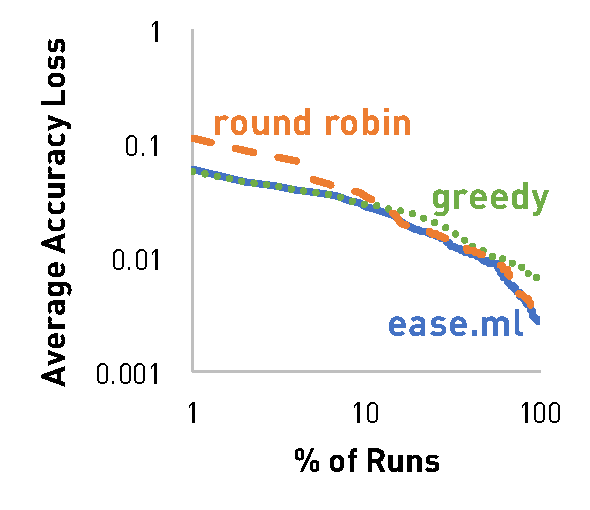
\includegraphics[width=0.25\textwidth]{figures/classifier_hybrid}
\vspace{-1em}
\caption{The impact of hybrid execution.}
\label{fig:hybrid-exec}
\vskip -2ex
\end{figure}

Figure~\ref{fig:hybrid-exec} illustrates the impact of this hybrid approach (denoted as {\bf \eml} in the figure).
We use {\bf greedy} and {\bf round robin} to denote Algorithm~\ref{alg:mc-general} and its round-robin variant, respectively.
We observe that, while {\bf greedy} outperforms {\bf round robin} at the beginning, there is some crossover point as the algorithms proceed where {\bf round robin} becomes superior to {\bf greedy}.
Switching to {\bf round robin} after that crossover point makes the hybrid execution strategy naturally the best among the three algorithms.


\newpage
~
\newpage




\section{Experiments}\label{sec:experiments}

We present experimental evaluation results of the multi-tenant GP-UCB algorithm in this section.
We evaluate the algorithm on both real and synthetic datasets, and compare its performance with baseline approaches, including the round-robin GP-UCB algorithm discussed in Section~\ref{sec:multitenant:round-robin}, a strong baseline since it observes the same regret bound as the multi-tenant GP-UCB algorithm.

\subsection{Datasets}

\begin{figure}
\small
\begin{tabular}{c | r r | c c c}
\hline
{\bf Dataset} & {\bf \# Users} & {\bf \# Models} & {\bf Quality} & {\bf Cost} \\
\hline
\textsc{DeepLearning} & 22 & 8 & Real & Real \\
\textsc{179Classifier} & 121 & 179 & Real & Synthetic \\
\hline
\textsc{SYN(0.01,0.1)} & 200 & 100 & Synthetic & Synthetic \\
\textsc{SYN(0.01,1.0)} & 200 & 100 & Synthetic & Synthetic \\
\textsc{SYN(0.5,0.1)} & 200 & 100 & Synthetic & Synthetic \\
\textsc{SYN(0.5,1.0)} & 200 & 100 & Synthetic & Synthetic \\
\hline
\end{tabular}
\vspace{-1em}
\caption{Statistics of Datasets}
\label{tab:datasets}
\vskip -2ex
\end{figure}

\begin{figure}[t!]
\centering
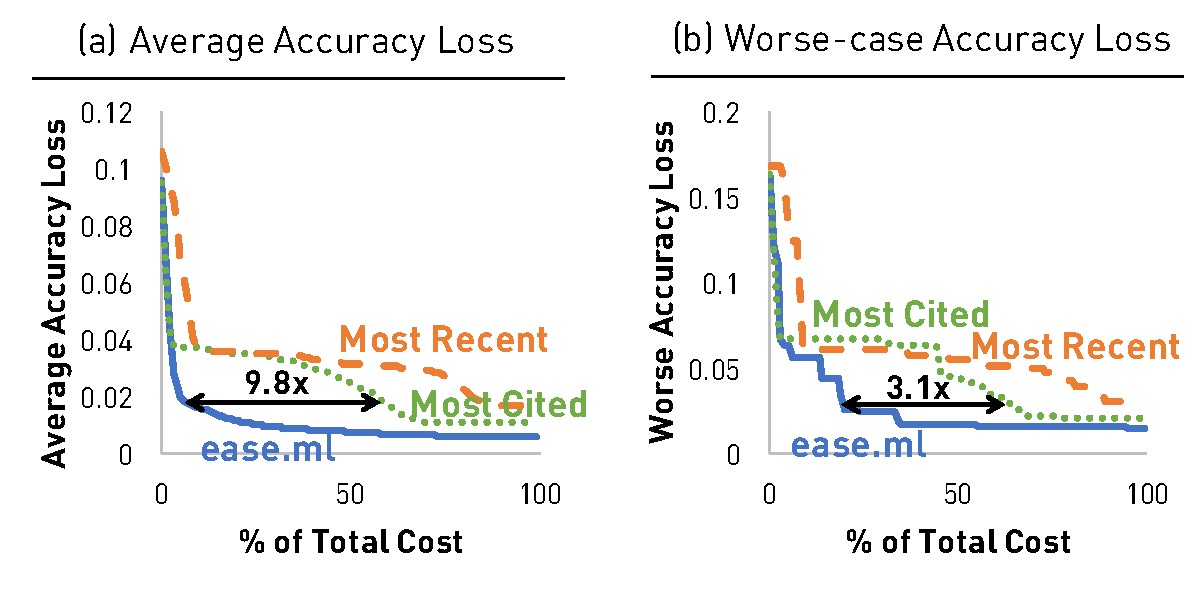
\includegraphics[width=0.4\textwidth]{figures/main}
\vspace{-2em}
\caption{End-to-end performance of
\texttt{ease.ml} on the
\textsc{DeepLearning} dataset
compared with two strategies
popularly used by our users 
without \texttt{ease.ml}--- (1) most cited network first; and (2) most recently
published network first.}
\label{fig:end-to-end}
\vskip -2ex
\end{figure}


Figure~\ref{tab:datasets} summarizes the datasets we used in our evaluation.
We employ two real datasets ``{\bf DeepLearning}'' and ``{\bf 179Classifier}'':
\vspace{-0.5em}
\begin{itemize}
\item {\bf DeepLearning} represents a workload with 22 users and 8 models that are all deep neural networks.
It is harvested from the real scenario as was depicted in the motivating example (Section~\ref{sec:introduction}).
We also have real statistics about costs of training these neural networks.
\vspace{-0.5em}
\item {\bf 179Classifier} represents a workload with 121 users and 179 models. The details of the user datasets and models can be found in~\cite{DelgadoCBA14}, where the datasets are collected from the UCI Machine Learning Repository~\cite{Lichman:2013}. We generate synthetic costs from the uniform distribution $\mathcal{U}(0, 1)$.
\end{itemize}
\vspace{-0.5em}
To understand the performance of the algorithms under more diverse workloads, we further evaluate them over synthetic datasets.
In the following, we briefly describe the synthetic data generator.

\subsubsection{Synthetic Data Generation}\label{sec:experiments:datagen}

We present the algorithm we used to generate synthetic data for $N$ users and $M$ models.
Our goal is to develop a generative model for the quality $x_{i,j}$ of a model $j\in[K]$ for a user $i\in[N]$.
We consider the following two factors that can affect $x_{i,j}$.

\vspace{-0.5em}
\begin{itemize}
\item {\bf User baseline quality} $b_i$: Different users have different
      hardness associated with their tasks --- we can achieve higher accuracy on some tasks than the others.
      For a user $i$, $b_i$ then describes how difficult the corresponding task is.
      In other words, $b_i$ characterizes the inherent hardness of $i$ and the model quality $x_{i,j}$ can be thought of as fluctuation around $b_i$ (for the model $j$).
      We simply draw the $b_i$'s from a normal distribution $\mathcal{N}(\mu_b,\sigma_b^2)$.
\vspace{-0.5em}
\item {\bf Model quality variation} $m_j$: Following the previous view of treating $x_{i,j}$ as fluctuation around $b_i$, we now use $m_j$ to denote this fluctuation for the model $j$. The next question is how to generate the $m_j$'s. Since different models may exhibit similar performance on a dataset (for example, linear models may perform similarly on a dataset conforming to a linear hypothesis space), the generative model for the $m_j$'s needs to capture this model correlation.
Therefore, rather than drawing the $m_j$'s independently, we specify their \emph{joint} distribution and draw the $m_j$'s simultaneously from the joint distribution.
Specifically, for each model $j$, we assign a score 
$$f(j)\sim\mathcal{U}(0,1),$$
where $\mathcal{U}$ represents the uniform distribution as before.
Given two models $j$ and $j'$, we define their similarity as
$$\Sigma_M[j, j']=\exp \left\{-\frac{(f(j) - f(j'))^2}{\sigma_M^2} \right\},$$
where $\sigma_M$ is a free parameter. We then sample
\[
[m_1,...,m_K] \sim \mathcal{N}(0, \Sigma_M).
\]
\end{itemize}
\vspace{-0.5em}

With the above discussion and notation, we can now define
\begin{equation}\label{eq:quality:simple}
x_{i,j} = b_i + \alpha\cdot m_j,
\end{equation}
where $\alpha\in(0,1]$ represents the relative impact of $m_j$ with respect to $b_i$.
By convention we define $x_{i,j}=0$ if Equation~\ref{eq:quality:simple} leads to $x_{i,j}<0$ and define $x_{i,j}=1$ if Equation~\ref{eq:quality:simple} leads to $x_{i,j}>1$.
We use $\SYN(\sigma_M, \alpha)$ to represent a synthetic dataset generated by using the two free parameters $\sigma_M$ and $\alpha$.
Figure~\ref{tab:datasets} lists the four synthetic datasets used in our evaluation. %with varying values of $\sigma_M$ and $\alpha$.

Note that here we have implicitly assumed that model correlation is independent of user datasets, that is, the same covariance matrix $\Sigma_M$ representing model correlation is used for all users.
This is, however, a simplified assumption.
It is possible that model correlation may vary across different user datasets.
We postpone discussion of a more general data generator to Appendix~\ref{sec:appendix:synthetic} that allows for using different model covariance matrices for different users.


\subsection{End-to-End Evaluation of ease.ml}

Finally, we present an end-to-end evaluation of {\bf \eml} on the {\bf DeepLearning} dataset, comparing against two heuristic strategies that are popularly employed in practice by our users: (1) most cited network first ({\bf most cited}); and (2) most recently published network first ({\bf most recent}).
These heuristics may sound amusing, however, they are reasonable from the viewpoint of scientists outside the computer science area.
\vspace{-0.5em}


Figure~\ref{fig:end-to-end} presents the comparison results in terms of accuracy loss.
We observe that {\bf \eml} can outperform the best of the two heuristics by an order of magnitude when comparing the average accuracy loss: The time spent on taking the average accuracy loss down from 0.1 to 0.02 of {\bf most cited} is about 9.8 times of (i.e., 8.8 times longer than) that of {\bf \eml}.
The gap drops to 3.1 times when comparing the worst-case accuracy losses.



\subsection{Performance of Multi-tenant GP-UCB}

We compare {\bf \eml} (i.e., Algorithm~\ref{alg:mc-general}) with two baseline approaches: {\bf random} and {\bf round robin}.
Similar to Algorithm~\ref{alg:mc-general}, both approaches consist of a user selection phase and a model selection phase at each time step.
The model selection phase remains the same: We use GP-UCB in the model selection phase for the selected user.
The user selection phases are different: (1) {\bf random} --- randomly pick the next user; and (2) {\bf round robin} --- pick the next user in a round-robin manner.
Recall that we have shown {\bf round robin} observes the same regret bound as {\bf \eml}. %(Section~\ref{sec:multitenant:round-robin}).

%\vspace{-0.5em}
\subsubsection{Experimental Settings}

GP-UCB requires to specify a prior $(\mu(\mathbf{x}), k(\mathbf{x},\mathbf{x}'))$.
As a convention, for GP's not conditioned on data, we assume that $\mu=0$ without loss of generality~\cite{SrinivasKKS10}.
While we can use standard kernel functions for the $k$, we need to come up with a vector representation (i.e., the $\mathbf{x}$) for the models.
For this purpose, we randomly split a dataset into a ``training set'' and a ``testing set.''
We use the training set to compute a vector for each model as follows:
We first evaluate the model on each user in the training set to get its quality, and we then pack these qualities into a ``quality vector'' $\mathbf{x}$ indexed by the users.
In our experiments, we used 90\% data for training and 10\% data for testing.
We run each experiment 50 times by using different random splits of the data into training and testing sets.

Given a dataset, for each of the three algorithms, we report its \emph{accuracy loss} as time goes by.
For a user $i\in[n]$ and a time step $T$, let $a_{i,T}=\max_{1\leq t\leq T} a_{i,t}$ be the best accuracy of evaluating the selected models up to the time $T$, and let $a_i^{*}$ be the best accuracy that the user $i$ can achieve.
We define the accuracy loss of the user $i$ at the time $T$ as
\begin{equation}
l_{i,T}=a_i^{*}-a_{i,T}.
\end{equation}
Accordingly, we define the accuracy loss at the time $T$ to be the average accuracy loss of the users:
\begin{equation}\label{eq:accuracy-loss}
l_T=\frac{1}{n}\sum\nolimits_{i=1}^{n}l_{i,T}.
\end{equation}
Clearly $l_T\to 0$ as $T\to\infty$, if the multi-tenant model selection algorithm is regret-free (i.e., the best model for each user is eventually found).
Moreover, we have $l_{i,T}\leq r_{i,T}$, namely, the accuracy loss of each user is upper bounded by his/her instantaneous regret.

One may wonder why we report accuracy loss instead of regret.
The reason is that accuracy loss is a metric we care more in practice.
Recall the real scenario where the multi-tenant model selection algorithm is applied in our system (Section~\ref{sec:architecture}): At each time step $T$, a user is using the best model he/she has found so far (even if he/she is not scheduled at time $T$) for his/her task, rather than using the model being evaluated at time $T$!
Therefore, compared with regret, accuracy loss is closer in the sense of characterizing the real user ``happiness.''
On the other hand, regret is the standard metric when analyzing bandit algorithms.
Given that accuracy loss is upper bounded by instantaneous regret, the upper bounds for regret apply to accuracy loss as well.%, though it is an open question that if we can have tighter upper bound for accuracy loss.

%\vspace{-0.5em}
\subsubsection{The Cost-oblivious Case}

Figure~\ref{fig:exp:cost-oblivious} presents the results for the cost-oblivious case.
Each row in Figure~\ref{fig:exp:cost-oblivious} represents the results of the three participating algorithms on one dataset.
The first column shows the average accuracy loss (of the 50 runs of the same experiment) as the number of runs increases, whereas the second column shows the worst-case accuracy loss (among the 50 runs of the same experiment) as the number of runs increases.
The third column further shows the model quality distribution (i.e., the distribution of the $x_{i,j}$'s).

\begin{figure}[!htb]
\centering
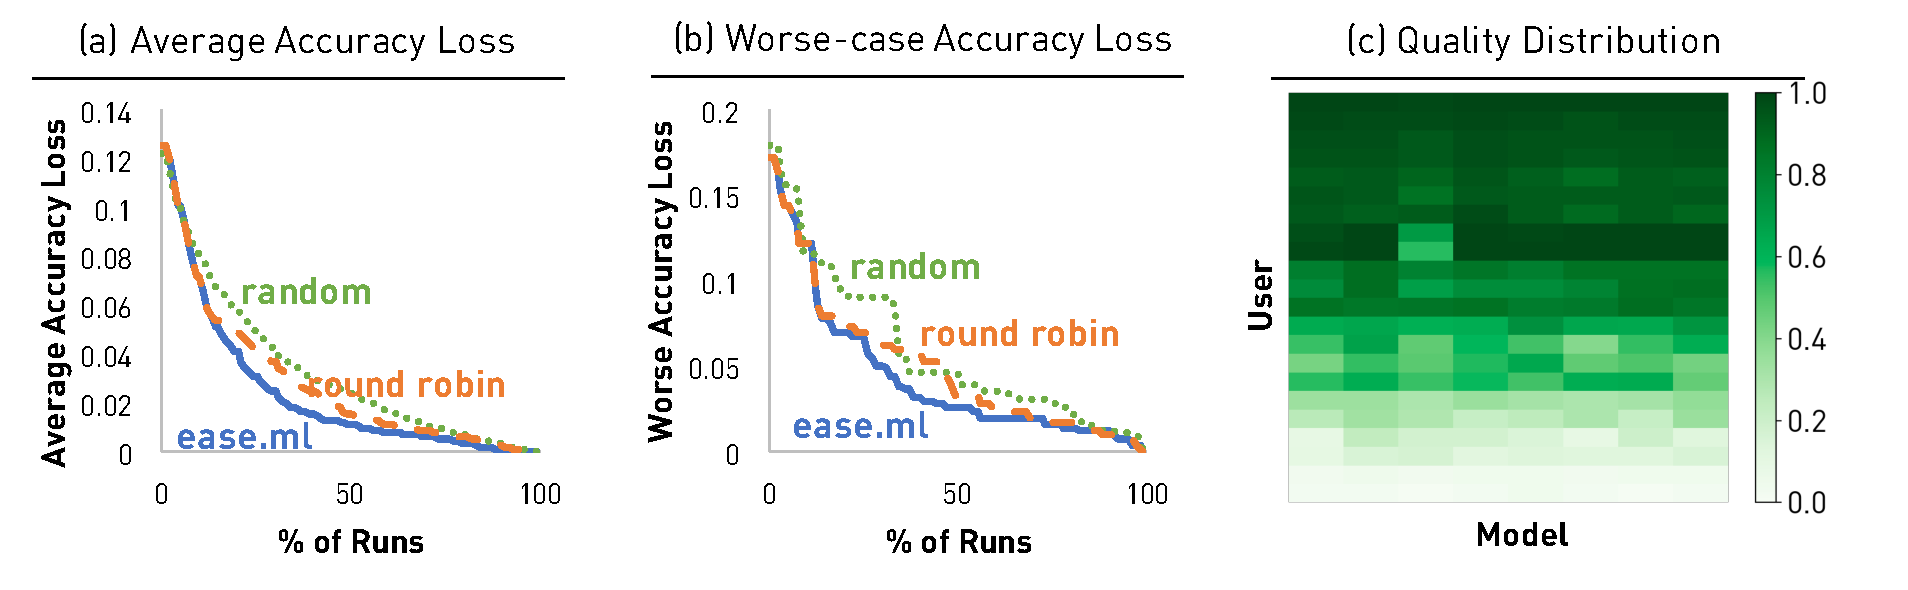
\includegraphics[width=0.5\textwidth]{figures/deeplearning_nocost}\\
\vspace{-0.5em}
\textsc{DeepLearning}\\
\vspace{0.5em}
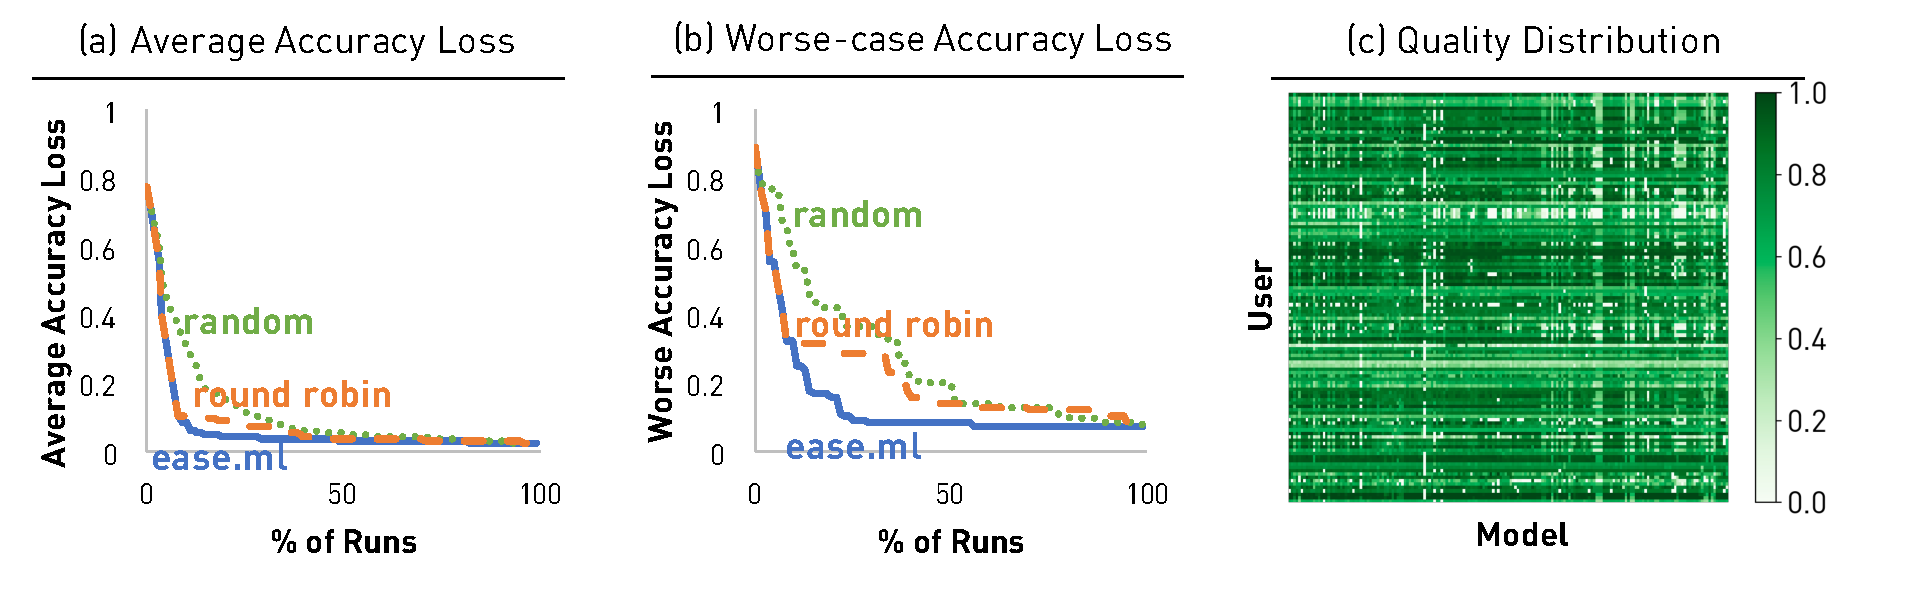
\includegraphics[width=0.5\textwidth]{figures/classifier_nocost}\\
\vspace{-0.5em}
\textsc{179Classifier}\\
\vspace{0.5em}
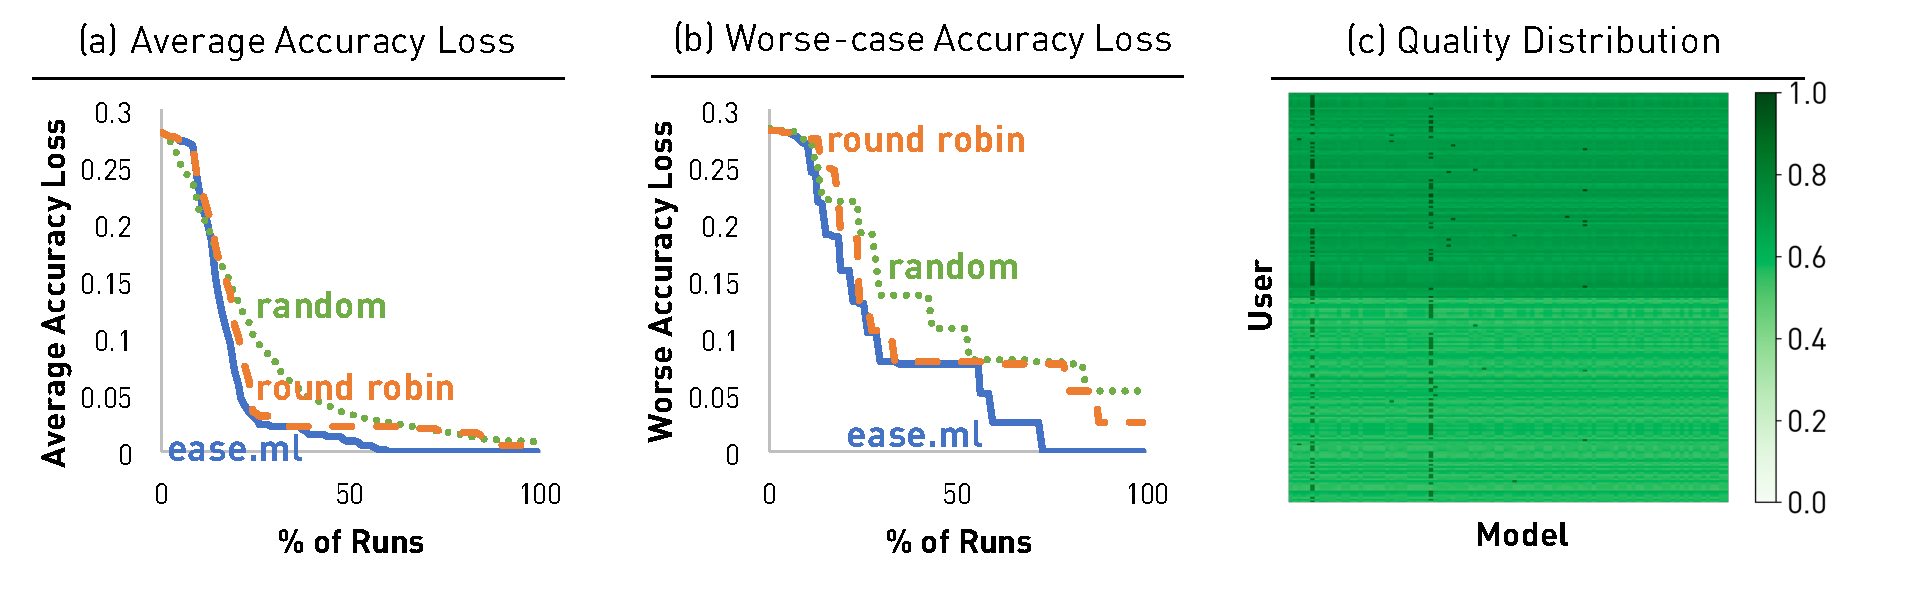
\includegraphics[width=0.5\textwidth]{{figures/syn_0.01_0.1_nocost}.pdf}\\
\vspace{-0.5em}
\textsc{SYN(0.01, 0.1)}\\
\vspace{0.5em}
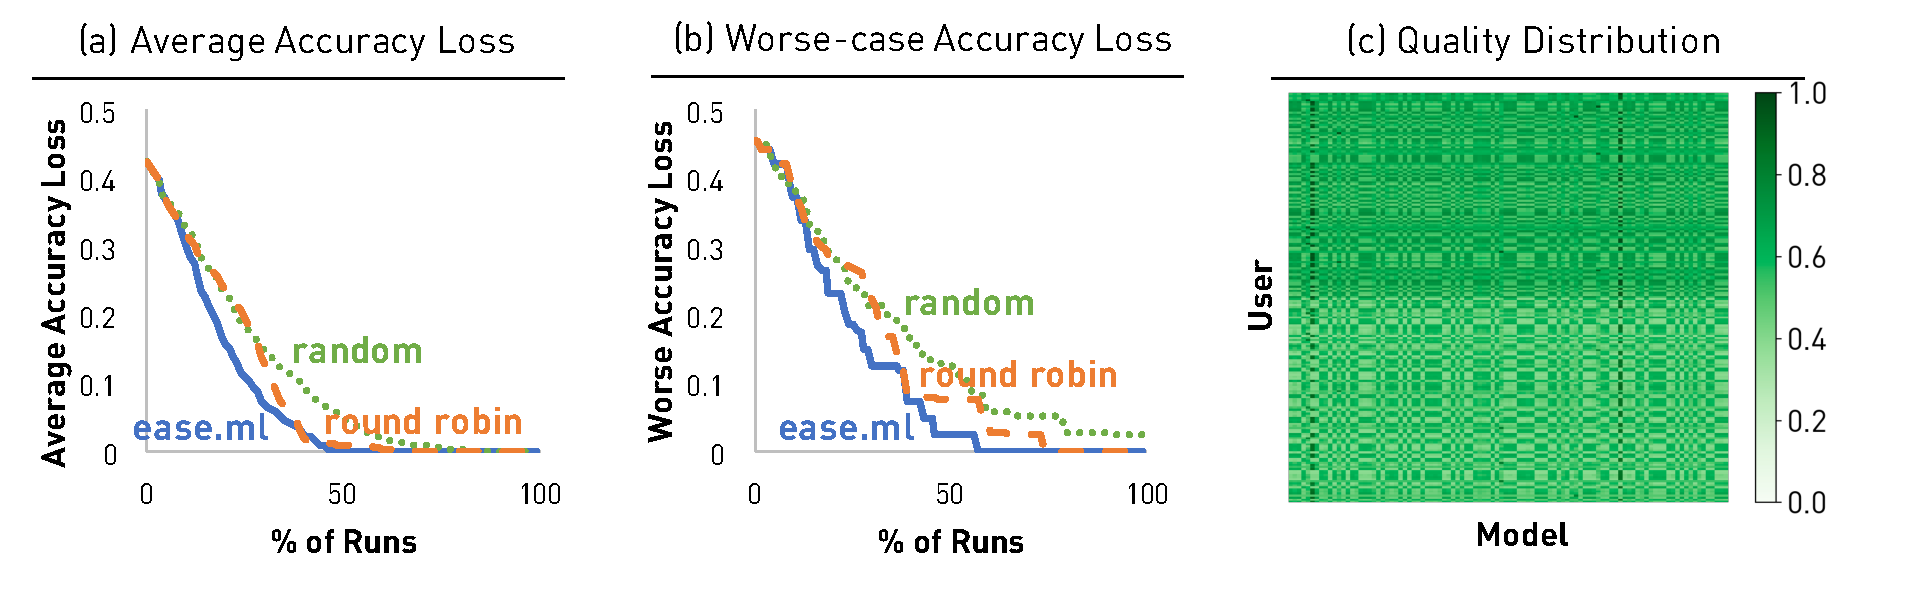
\includegraphics[width=0.5\textwidth]{{figures/syn_0.01_1.0_nocost}.pdf}\\
\vspace{-0.5em}
\textsc{SYN(0.01, 1.0)}\\
\vspace{0.5em}
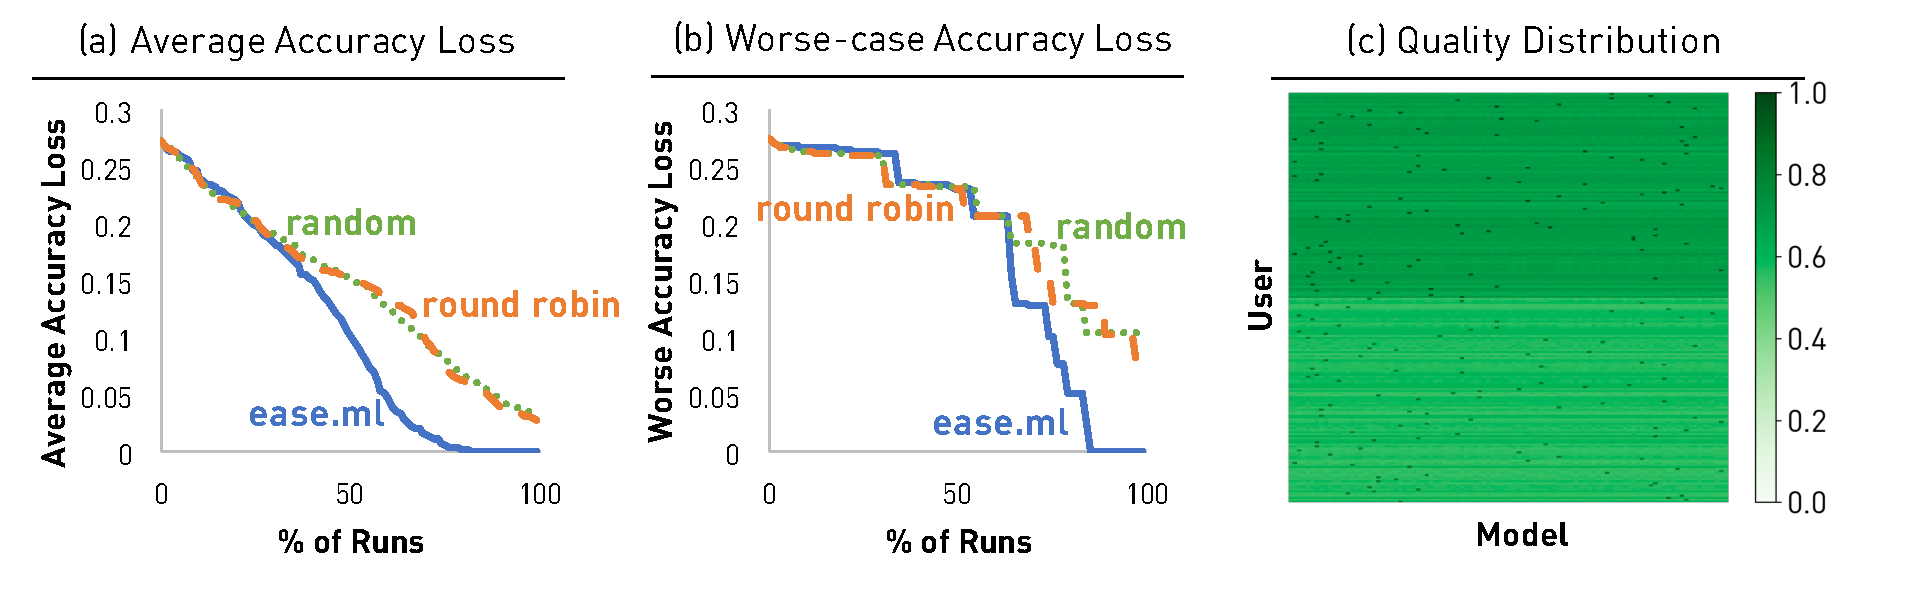
\includegraphics[width=0.5\textwidth]{{figures/syn_0.5_0.1_nocost}.pdf}\\
\vspace{-0.5em}
\textsc{SYN(0.5, 0.1)}\\
\vspace{0.5em}
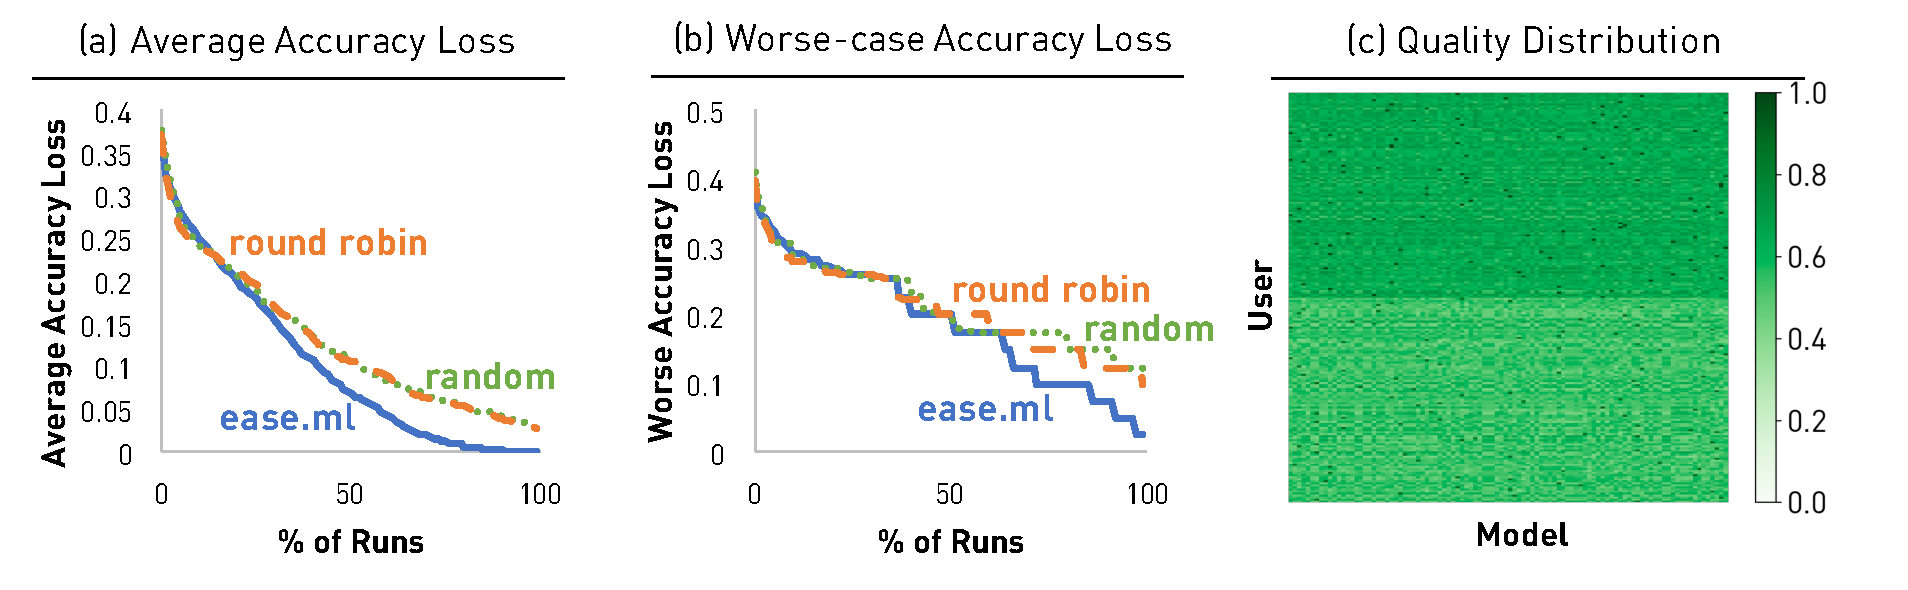
\includegraphics[width=0.5\textwidth]{{figures/syn_0.5_1.0_nocost}.pdf}\\
\vspace{-0.5em}
\textsc{SYN(0.5, 1.0)}
\vspace{-0.5em}
\caption{Performance of the cost-oblivious case.}
\label{fig:exp:cost-oblivious}
\vskip -4ex
\end{figure}

On the two real datasets {\bf DeepLearning} and {\bf 179Classifier}, we observe that both the average and the worst-case accuracy loss of {\bf \eml} drop (often much) faster compared with {\bf random} and {\bf round robin}, whereas {\bf round robin} also outperforms {\bf random}.
This implies that, {\bf \eml} reduces the total regret of all users faster than the other two baselines, and this performance is robust against different training and testing sets.

%The former is understandable. After all, {\bf \eml} is designed to minimize the total regret.
%The latter, however, is not presumed.
%The fact that {\bf \eml} can quickly reduce the maximum regret is essentially a consequence of the user selection strategy it employs. 
%{\color{red} Recall that {\bf \eml} always picks a user with above-average uncertainty and maximum expected improvement, therefore the user with %the maximum regret can be selected with high probability.}

The same pattern retains on the synthetic datasets: {\bf \eml} consistently beats {\bf random} and {\bf round robin}.
We do observe the impact of model correlation on the performance of the algorithms, though.
In Figure~\ref{fig:impact-model-correlation}, we present more detailed analysis from this aspect.
As we increase $\sigma_M$ from 0.01 to 0.5, the model correlation increases; as we reduce $\alpha$ from 1.0 to 0.1, the impact of model correlation decreases, which implies that the impact of the model-irrelevant noise (i.e., the user baseline quality) increases.
As is illustrated in Figure~\ref{fig:impact-model-correlation}, the performance of the algorithms improves upon stronger model correlation.
This is understandable: When model correlation becomes stronger, it is easier to distinguish good models from bad ones.
On the other hand, consider an extreme case when all the models are independent.
In such circumstance, evaluation of one model cannot gain information about the others, which therefore requires more exploration before the overall picture of model performance becomes clear.
Meanwhile, dampening the impact of model correlation has similar effects.

%\vspace{-0.5em}
\subsubsection{The Cost-aware Case}

Figure~\ref{fig:exp:cost-aware} presents the performance of the three algorithms in the cost-aware case.
For the {\bf DeepLearning} dataset, we use the real cost statistics.
For the {\bf 179Classifier} dataset and the four synthetic datasets, we generate costs randomly from the distribution $\mathcal{U}(0,1)$.

\begin{figure}
\centering
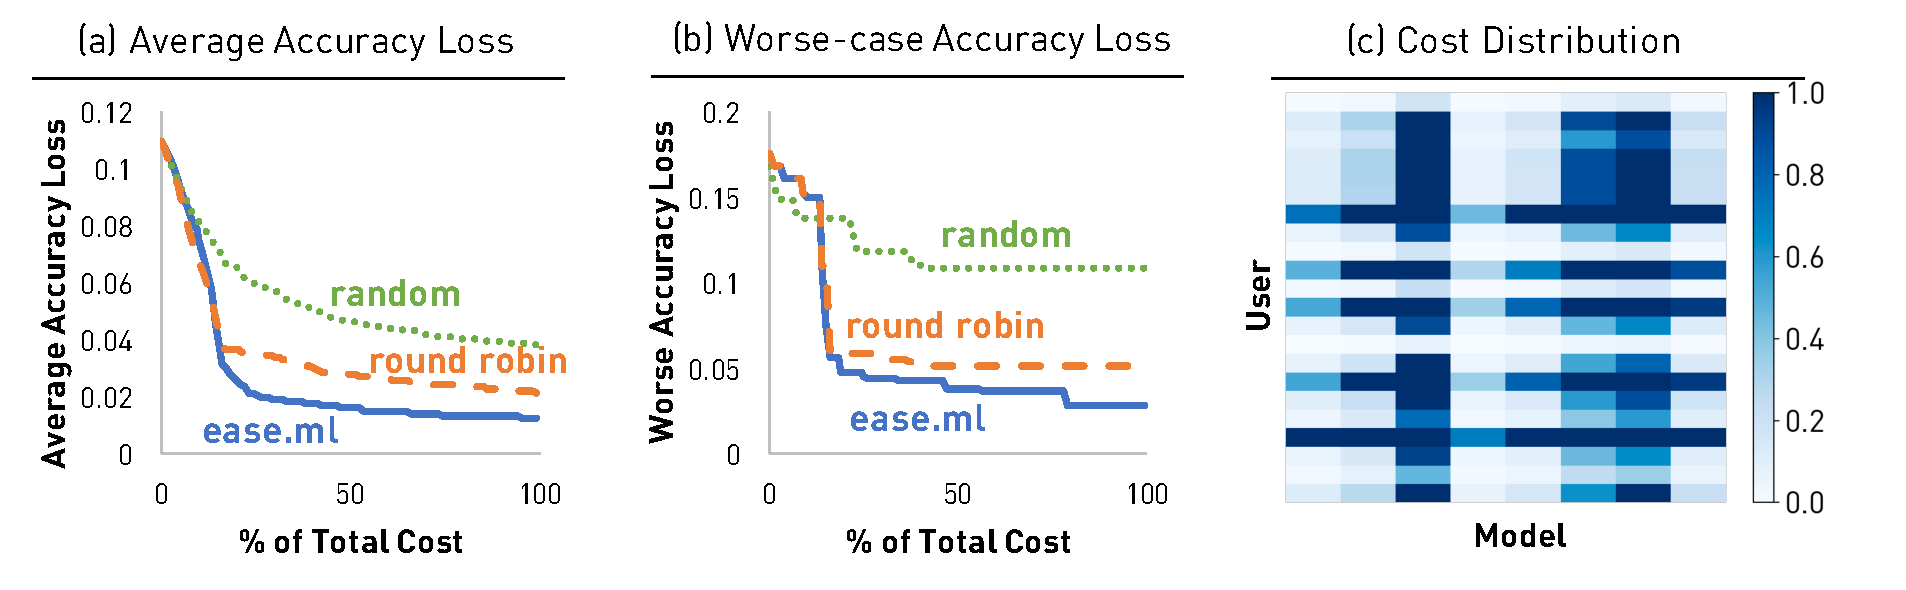
\includegraphics[width=0.5\textwidth]{figures/deeplearning_cost}\\
\vspace{-0.5em}
\textsc{DeepLearning}\\
\vspace{0.5em}
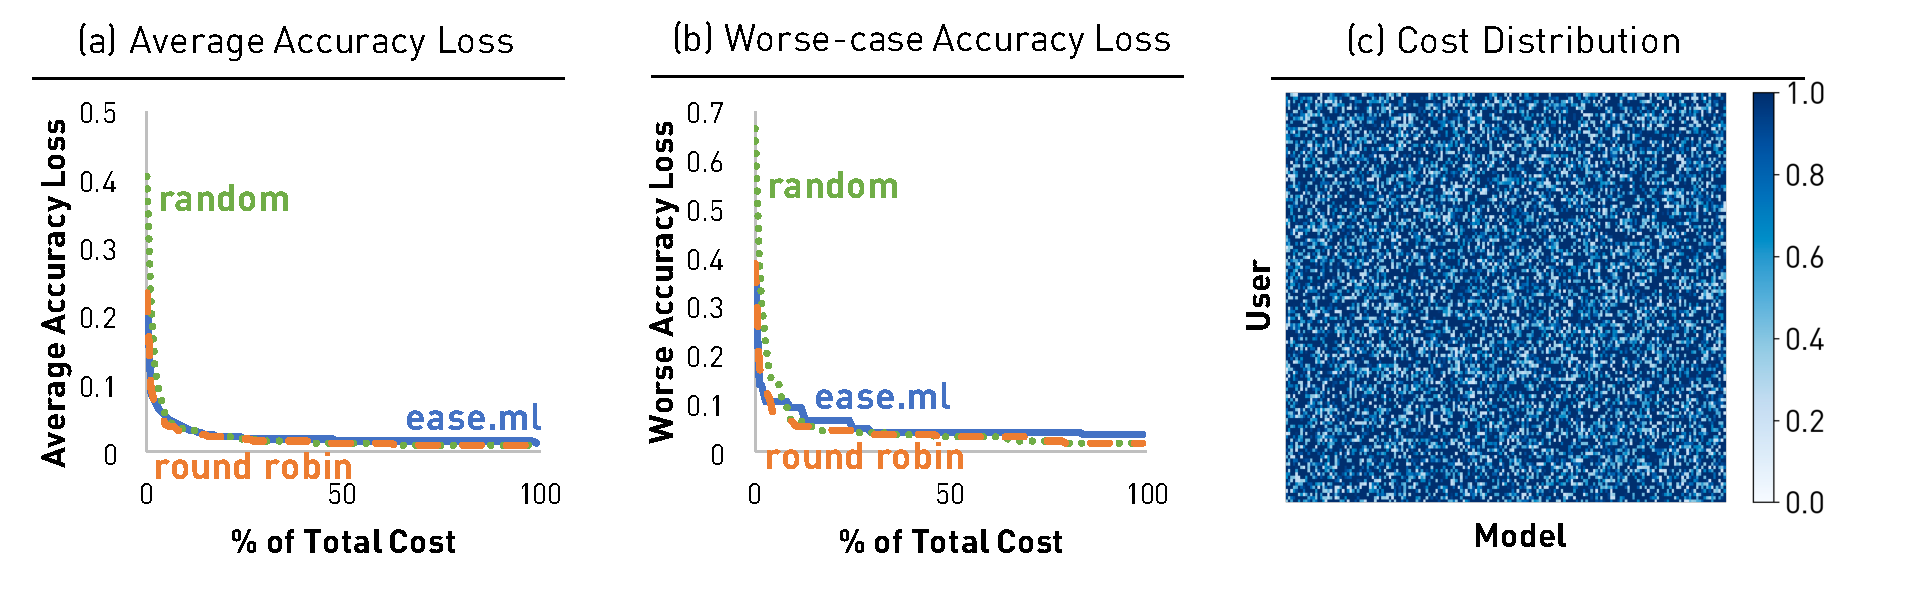
\includegraphics[width=0.5\textwidth]{figures/classifier_cost}\\
\vspace{-0.5em}
\textsc{179Classifier}\\
\vspace{0.5em}
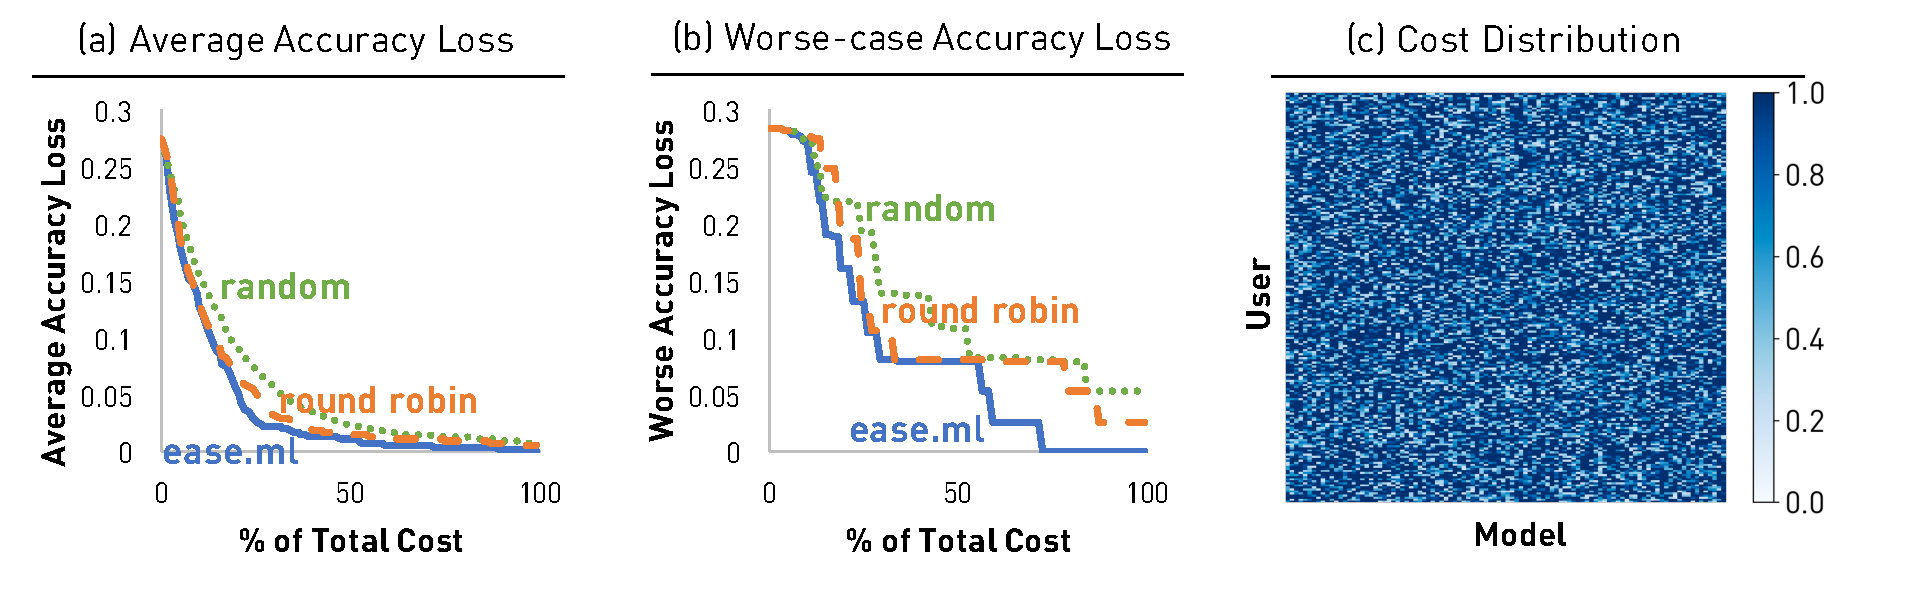
\includegraphics[width=0.5\textwidth]{{figures/syn_0.01_0.1_cost}.pdf}\\
\vspace{-0.5em}
\textsc{SYN(0.01, 0.1)}\\
\vspace{0.5em}
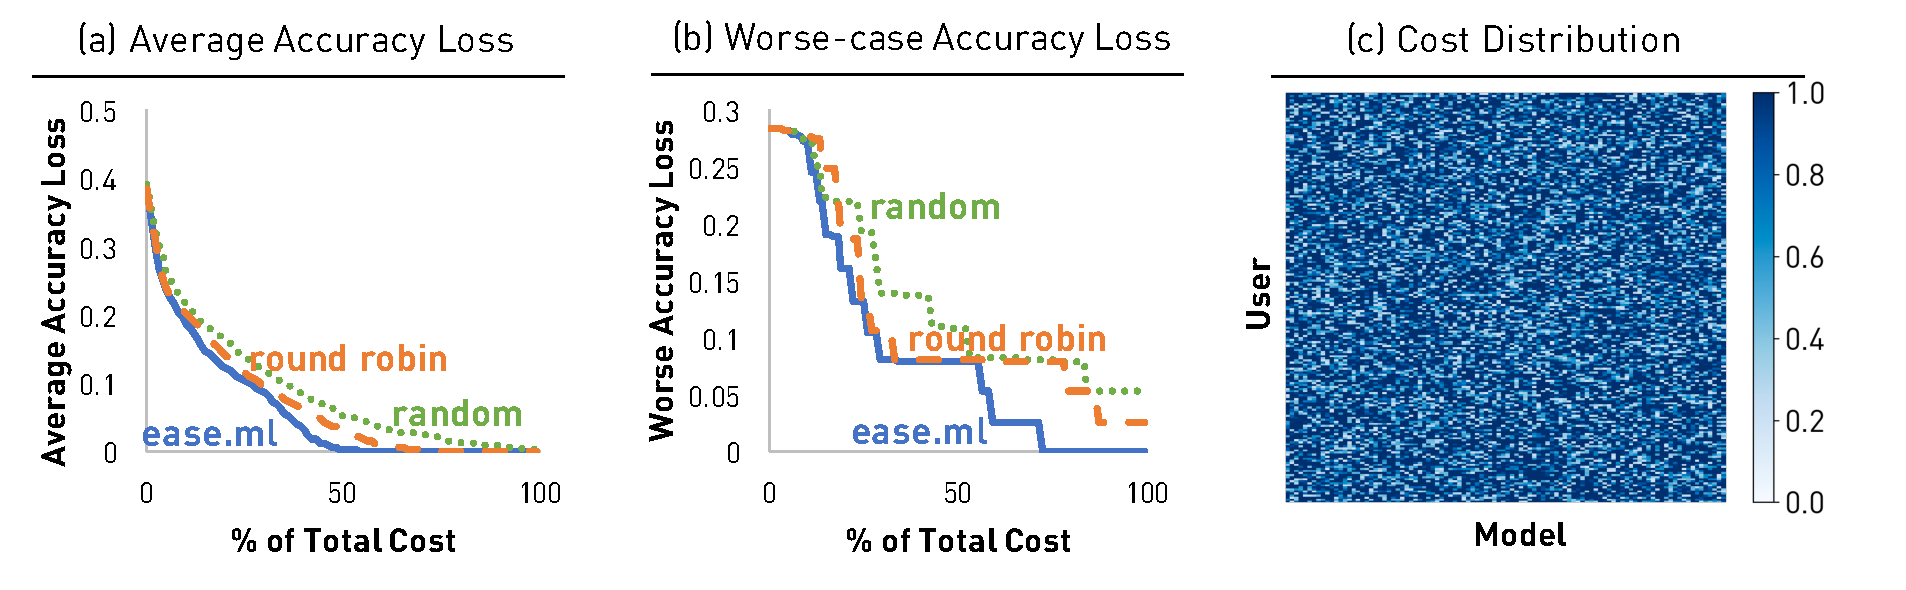
\includegraphics[width=0.5\textwidth]{{figures/syn_0.01_1.0_cost}.pdf}\\
\vspace{-0.5em}
\textsc{SYN(0.01, 1.0)}\\
\vspace{0.5em}
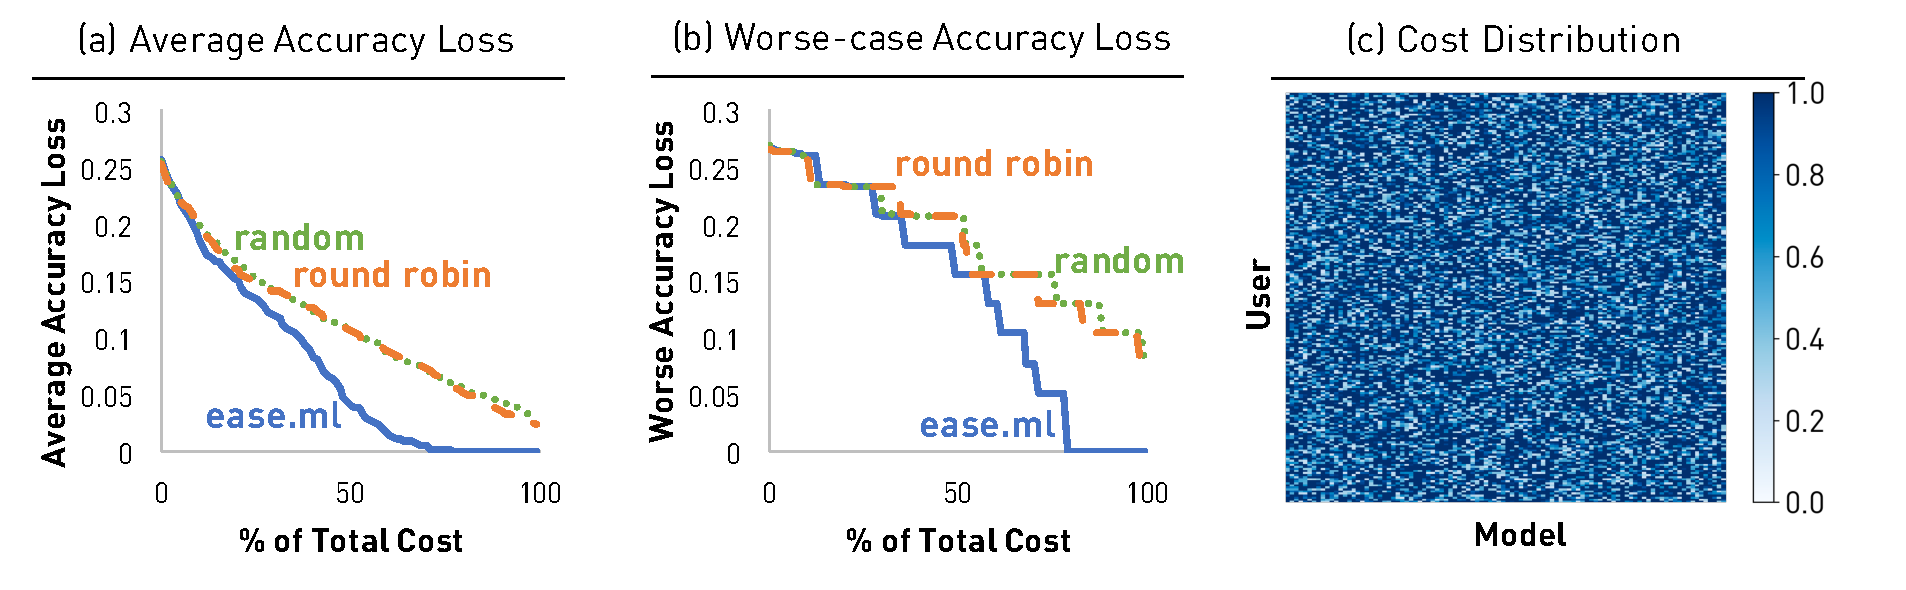
\includegraphics[width=0.5\textwidth]{{figures/syn_0.5_0.1_cost}.pdf}\\
\vspace{-0.5em}
\textsc{SYN(0.5, 0.1)}\\
\vspace{0.5em}
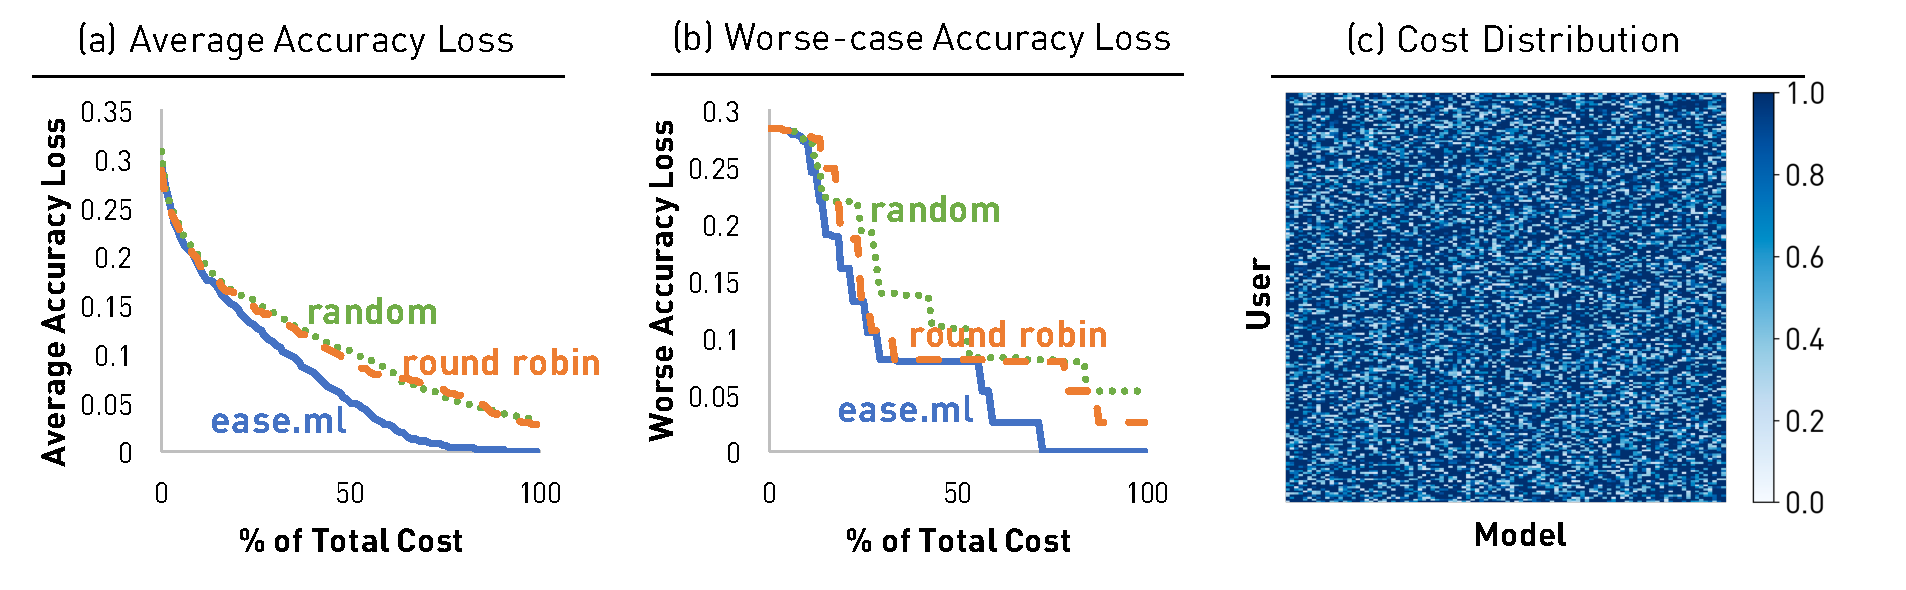
\includegraphics[width=0.5\textwidth]{{figures/syn_0.5_1.0_cost}.pdf}\\
\vspace{-0.5em}
\textsc{SYN(0.5, 1.0)}
\vspace{-0.5em}
\caption{Performance of the cost-aware case.}
\label{fig:exp:cost-aware}
\vskip -2ex
\end{figure}

The relative performance of the three algorithms is similar in the cost-aware case.
However, one may now have the question regarding the benefits of considering costs in model selection.
Figure~\ref{fig:impact-cost-aware} further compares the performance of {\bf \eml} in the cost-oblivious case and in the cost-aware case on the {\bf DeepLearning} dataset, where real cost statistics are available.
We observe huge performance improvement of the cost-aware {\bf \eml} over the cost-oblivious {\bf \eml}.
To achieve the same average/worst-case accuracy loss, it takes much longer in the cost-oblivious case.


\begin{figure*}[t]
\centering
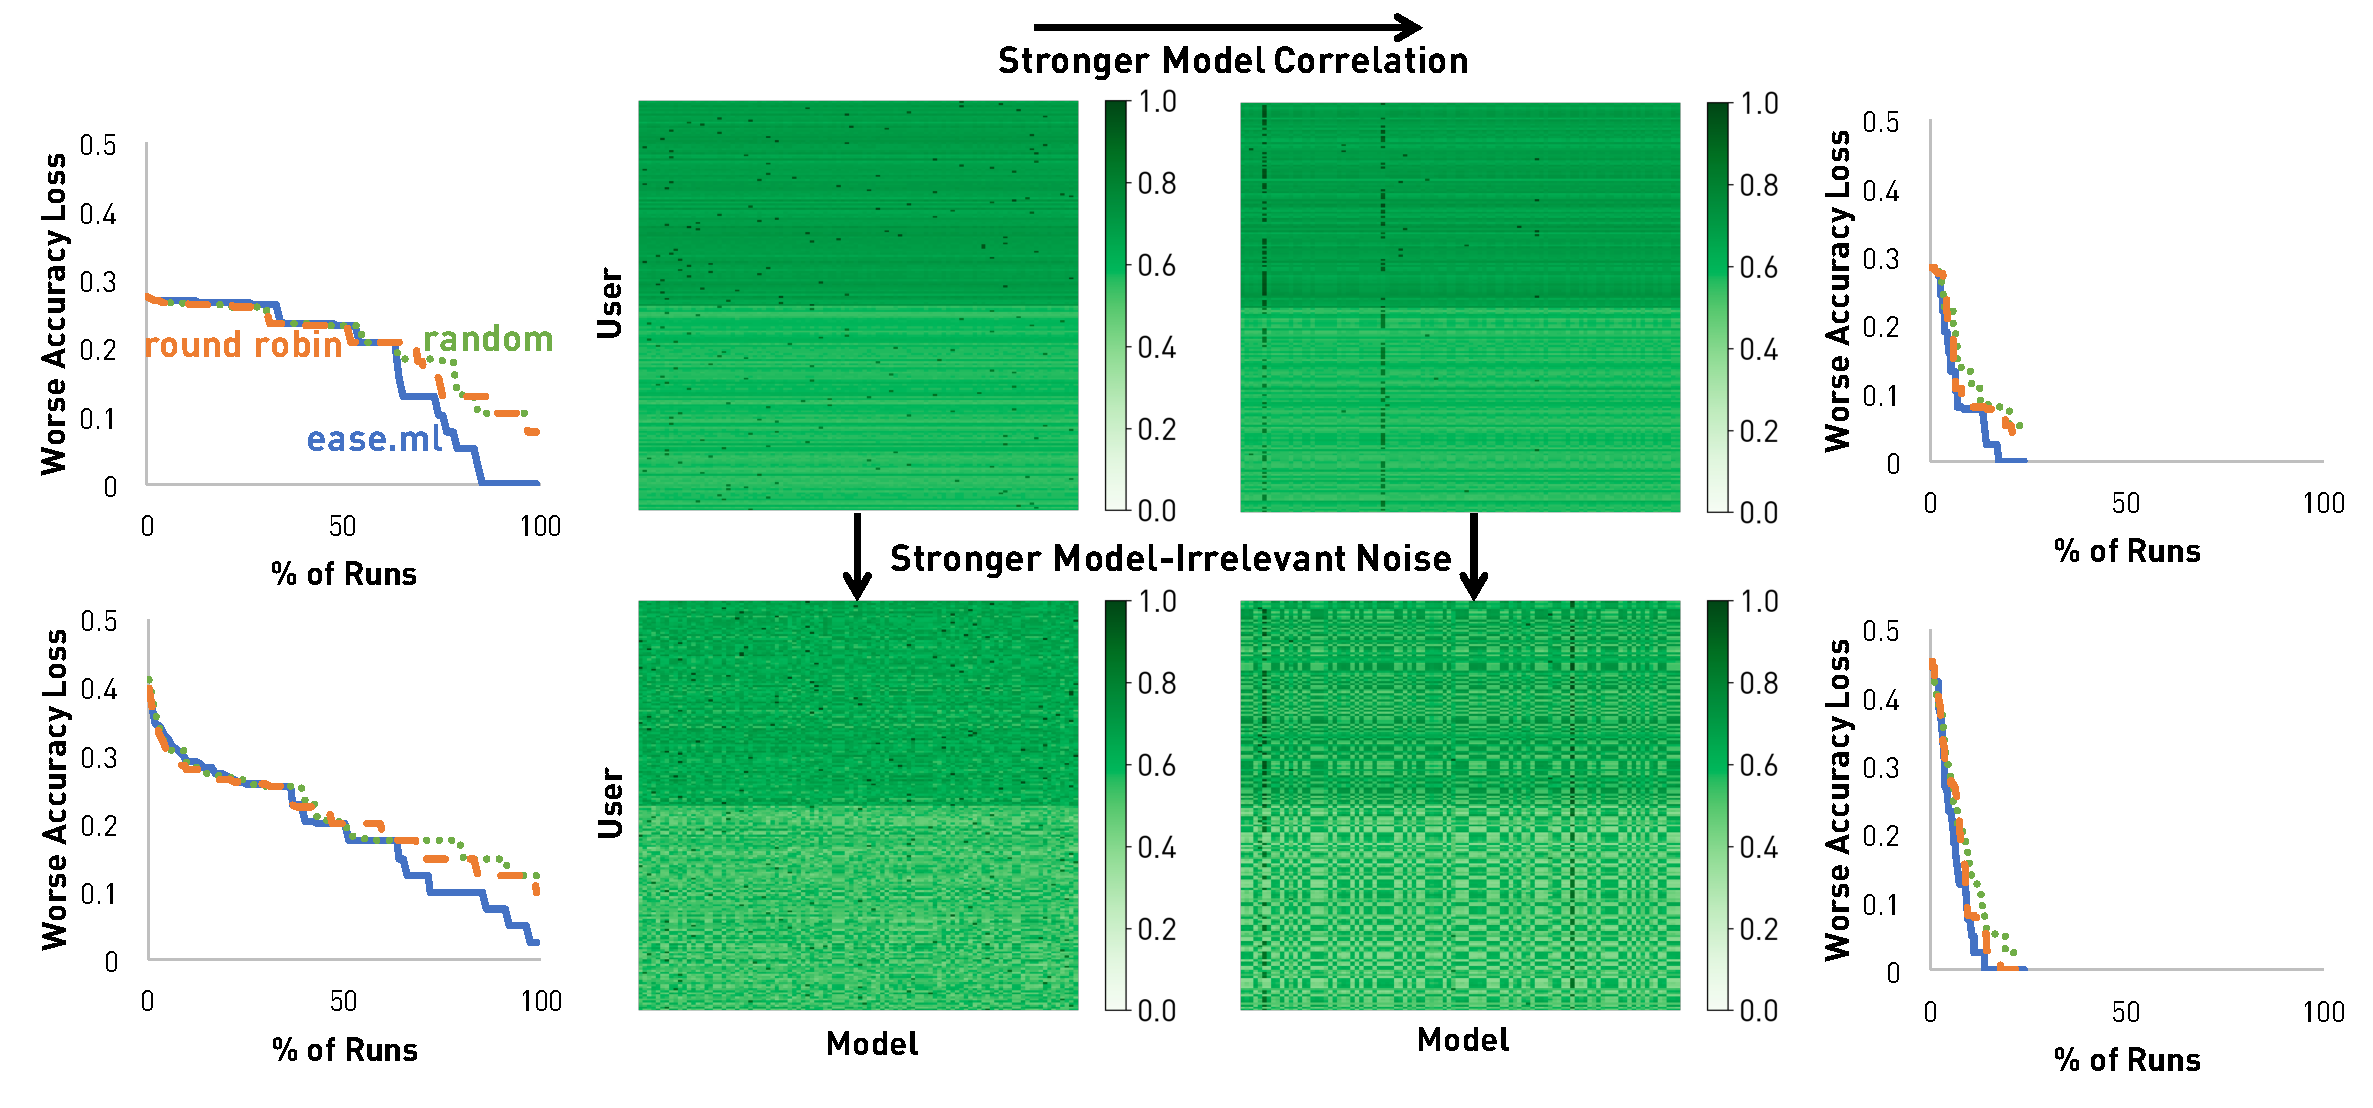
\includegraphics[width=0.8\textwidth]{figures/impact}
\vspace{-1em}
\caption{The impact of model correlation and noise: top left --- SYN(0.01, 1.0), top right --- SYN(0.5, 1.0), bottom left --- SYN(0.01, 0.1), and bottom right --- SYN(0.5, 0.1).}
\label{fig:impact-model-correlation}
\vskip -2ex
\end{figure*}


\begin{figure}
\centering
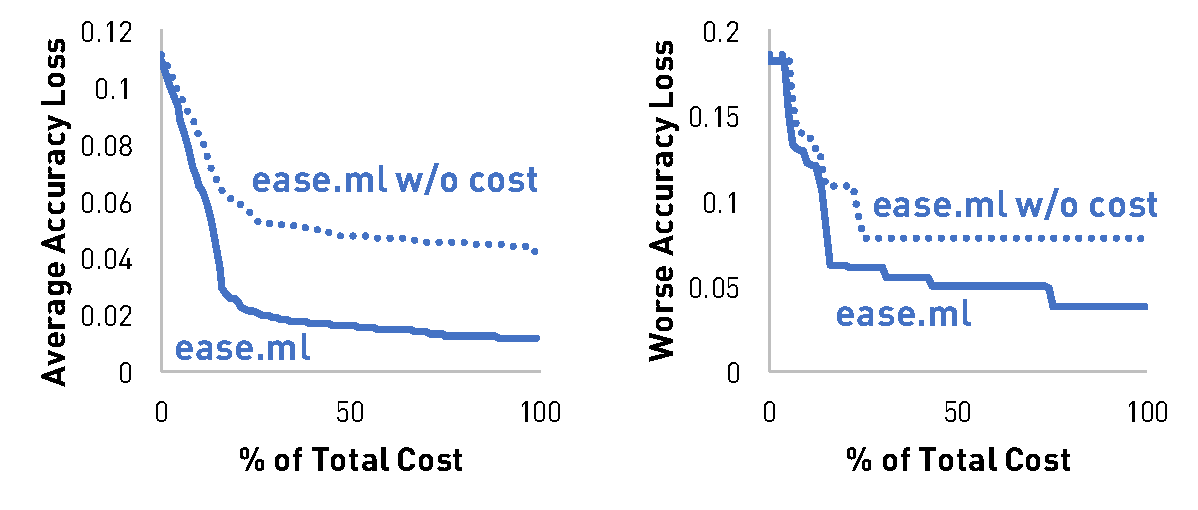
\includegraphics[width=0.33\textwidth]{figures/deeplearning_lesion}\\
\vspace{-0.75em}
\textsc{DeepLearning}\\
%\vspace{1em}
%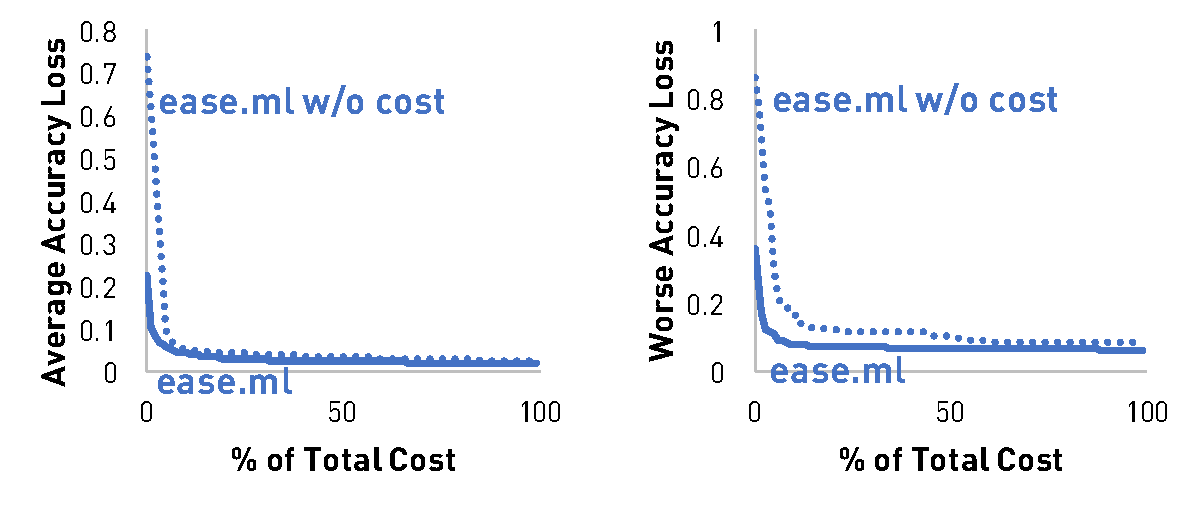
\includegraphics[width=0.33\textwidth]{figures/classifier_lesion}\\
%\vspace{-0.75em}
%\textsc{179Classifier}%\\
%\vspace{1em}
%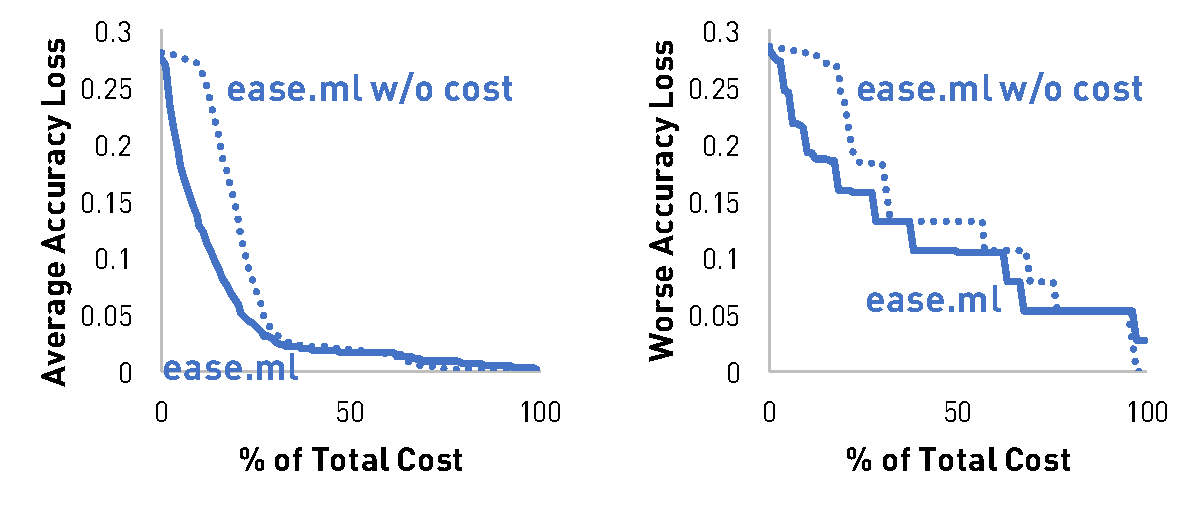
\includegraphics[width=0.33\textwidth]{{figures/syn_0.01_0.1_lesion}.pdf}\\
%\vspace{-0.75em}
%\textsc{SYN(0.01, 0.1)}\\
%\vspace{1em}
%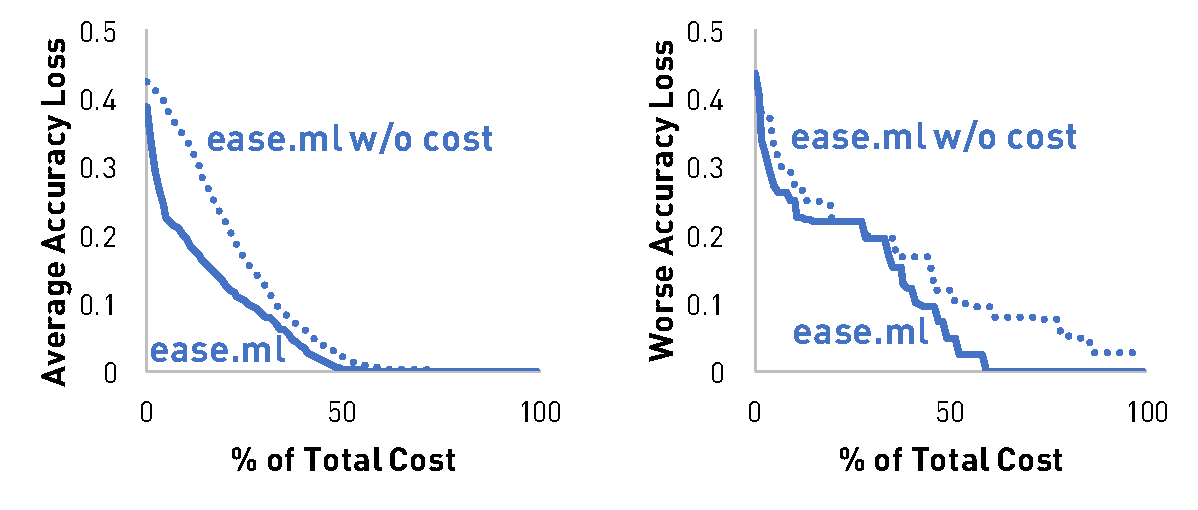
\includegraphics[width=0.33\textwidth]{{figures/syn_0.01_1.0_lesion}.pdf}\\
%\vspace{-0.75em}
%\textsc{SYN(0.01, 1.0)}\\
%\vspace{1em}
%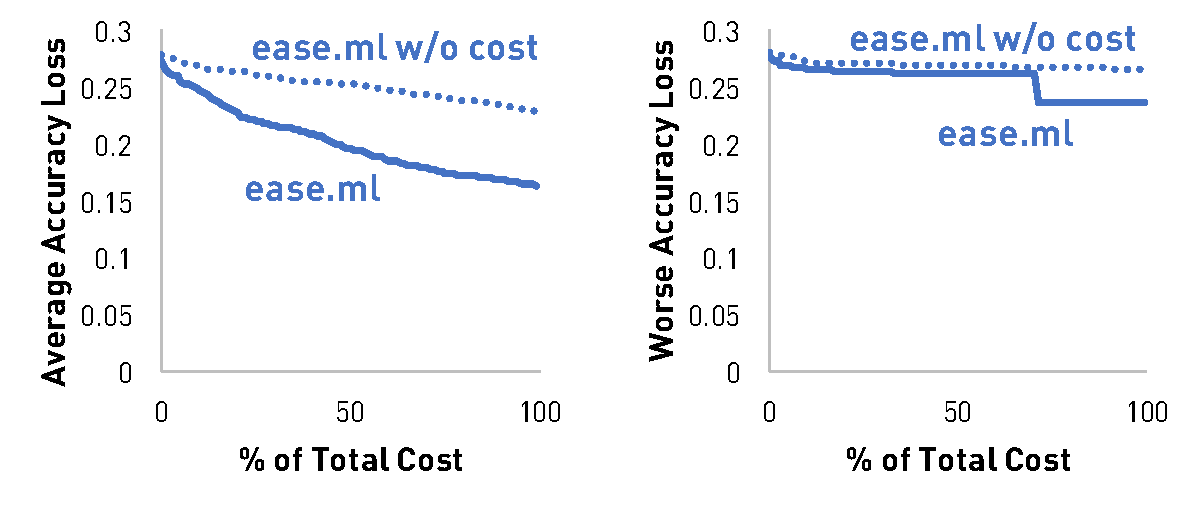
\includegraphics[width=0.33\textwidth]{{figures/syn_0.5_0.1_lesion}.pdf}\\
%\vspace{-0.75em}
%\textsc{SYN(0.5, 0.1)}\\
%\vspace{1em}
%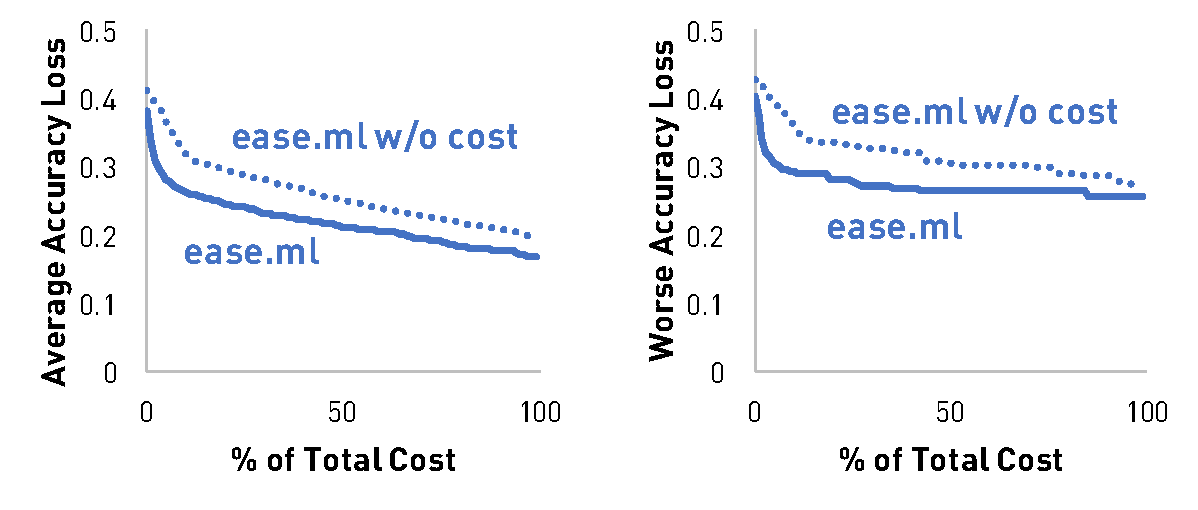
\includegraphics[width=0.33\textwidth]{{figures/syn_0.5_1.0_lesion}.pdf}\\
%\vspace{-0.75em}
%\textsc{SYN(0.5, 1.0)}
\vspace{-1em}
\caption{The impact of cost-awareness.}
\label{fig:impact-cost-aware}
\vskip -2ex
\end{figure}

\subsection{Impact of the Training Data Size}

Since the kernel of the GP prior is obtained from a training set, a natural question is how sensitive the performance of the algorithms is to the availability of training data.
To investigate this, we further study the impact of the training data size on the performance.
Figure~\ref{fig:training:oblivious} and~\ref{fig:training:aware} present the results in the cost-oblivious and cost-aware settings, respectively.

\begin{figure}
\centering
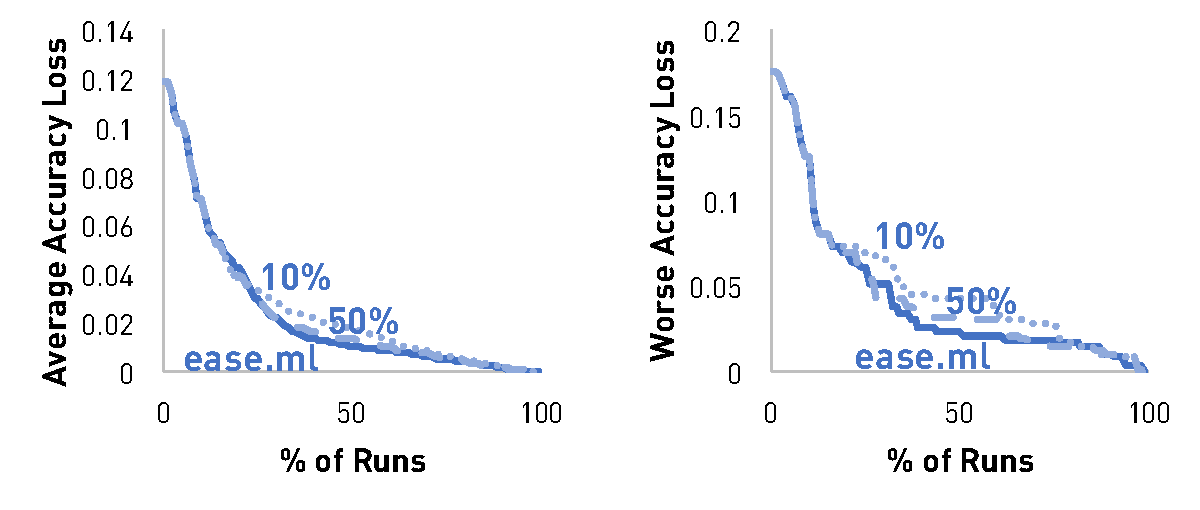
\includegraphics[width=0.33\textwidth]{figures/impact_train_nocost}
\vspace{-1em}
\caption{The impact of training set size (cost oblivious).}
\label{fig:training:oblivious}
\vskip -2ex
\end{figure}

\begin{figure}
\centering
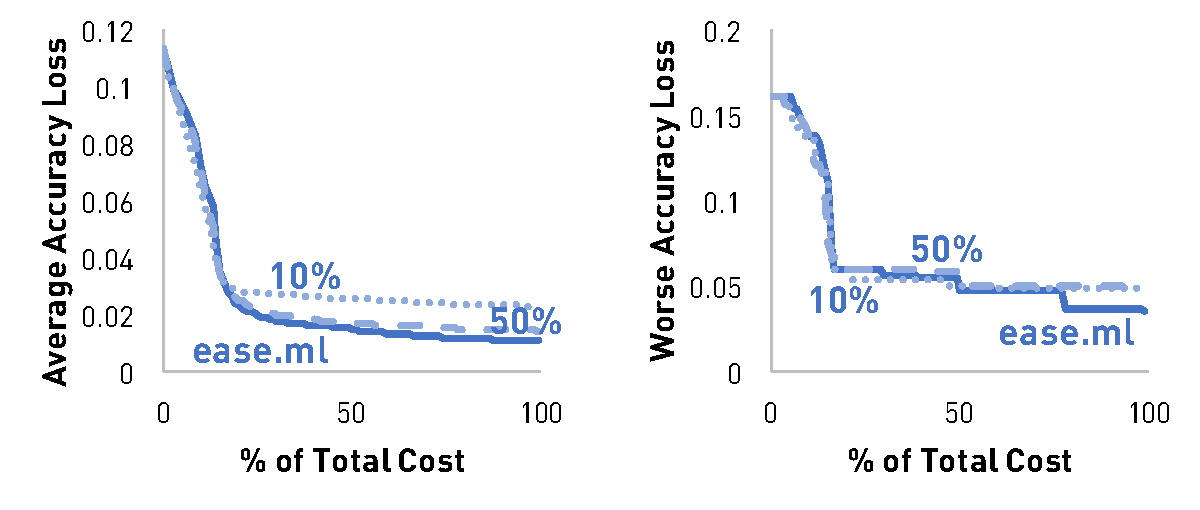
\includegraphics[width=0.33\textwidth]{figures/impact_train_cost}
\vspace{-1em}
\caption{The impact of training set size (cost aware).}
\label{fig:training:aware}
\vskip -2ex
\end{figure}

In our experiments, we varied the training data set size from 10\% to 100\% of the original training set size,
and we show the performance by using 10\%, 50\%, and 100\% training data.
We observe that using all training data is somehow unnecessary, as using only 50\% training data already achieves similar performance.
In fact, even if we only use 10\% training data, the performance is not much worse.
It is therefore convincing that {\bf \eml} can work well even if training data is scarce.


\section{Related Work}\label{sec:relatedwork}

The problem of automatic model selection and hyper-parameter tuning has been studied extensively. (See a recent survey by Luo~\cite{Luo16} for an overview of this area.)
Nonetheless, we are unaware of any work that considers the model selection problem in a multi-tenant setting.
The multi-tenancy circumstance is quite natural when hosting a shared machine learning infrastructure.

Our idea of viewing model selection as a multi-armed bandit problem is inspired by the recent work from Sparks et al.~\cite{SparksTHFJK15}, though the authors only considered the single-tenant model selection problem.
Historically, the study of the bandit problem can date back to the time of World War II~\cite{Robbins:1952}.
In the seminal paper by Lai and Robbins~\cite{Lai:1985}, the authors first introduced a class of algorithms based on UCBs that possess the fastest rate of convergence.
Agrawal~\cite{Agrawal1995} and Auer~\cite{Auer02,Auer:2002} further proposed more tractable versions of the UCB algorithm with similar regret bounds.
The GP-UCB algorithm comes from a relatively recent development by Srinivas et al.~\cite{SrinivasKKS10} where they introduced Bayesian optimization into the UCB algorithm.
Compared with other solutions to the bandit problem that are based on heuristic metrics such as probability of improvement (PI)~\cite{Kushner1964}, expected improvement (EI)~\cite{SnoekLA12}, or Thompson sampling~\cite{ChapelleL11,KaufmannKM12,Scott:2010},
the UCB algorithms are favourable due to their theoretically provable regret bounds.
However, none of them has ever considered the aspect of cost in terms of playing arms or model selection, which is essential in the multi-tenancy setting.

\paragraph*{Multitenant Clouds and Resource Management}

\paragraph*{Machine Learning Clouds}

\paragraph*{Multi-armed Bandits for Systems}

\paragraph*{Learning Curve Estimation}

\paragraph*{Automatic Model Selection}

\paragraph*{Automatic Hyperparameter Tuning}

\section{Conclusion}\label{sec:conclusion}

In this paper, we present the architecture of \eml, a declarative machine learning system that automatically manages an infrastructure shared by multiple users.
We focused on studying one of the key technical problems in \eml, the what we called multi-tenant model selection problem.
We gave the first problem formulation and proposed a solution that extends the well-known GP-UCB algorithm into the general multi-tenant, cost-aware setting.
We further showed that the total regret of the users can be bounded by $O(\sqrt{T})$, which is in line with the best known bound for the standard single-tenant GP-UCB algorithm.
Experimental evaluation substantiates the effectiveness of \eml, which significantly outperforms popular heuristic approaches currently used in practice as well as a strong round-robin baseline algorithm that observes the same $O(\sqrt{T})$ regret bound.

%\newpage
\bibliographystyle{abbrv}
\bibliography{vldb_sample}  



%\newpage 
\appendix

\section{Details of Synthetic Data Generation}\label{sec:appendix:synthetic}

We present the algorithm we used to generate synthetic data for $N$ users and $M$ models.
We assume that the quality of a model $j\in[M]$ for a user $i\in[N]$ can be decomposed into the following four factors:

\vspace{-0.5em}
\begin{enumerate}
\item {\bf User baseline quality} $b_i$: Different users have different
      hardness associated with their tasks --- we can achieve higher accuracy on some tasks than the others.
      For a user $i$, $b_i$ then describes how difficult the corresponding task is.
\vspace{-0.5em}
\item {\bf Model quality correlation} $m_j$: For each user $i$, $\{m_j\}$ corresponds to the fluctuation of the quality of the model $j$ over the baseline quality that can be explained by model correlation.
      For example, on a given user dataset, we would expect ResNet-20 always outperforms ResNet-50 if the dataset is small.
      %{\color{red} This factor tries to capture correlations between models.}
\vspace{-0.5em}
\item {\bf User quality correlation} $u_i$: For each model $j$, $\{u_i\}$ corresponds to the fluctuation of the quality of the model $j$ across different users
      over the baseline quality that can be explained by user dataset correlation.
      For example, given a neural network such as ResNet-1000, we should expect that it works well on all large datasets but worse on all small ones.
      %{\color{red} This factor tries to capture correlations between users.}
\vspace{-0.5em}
\item {\bf White noise} $\epsilon_{i,j}$: This factor tries to capture everything that are
      not explained by the previous three factors.
\end{enumerate}
\vspace{-0.5em}

Let $x_{i,j}$ be the quality of model $j$ for user $i$. With the above notation, it follows that
\begin{equation}\label{eq:quality}
x_{i,j} = b_i + m_j + u_i + \epsilon_{i,j}.
\end{equation}
By convention we define $x_{i,j}=0$ if Equation~\ref{eq:quality} leads to $x_{i,j}<0$ and define $x_{i,j}=1$ if Equation~\ref{eq:quality} leads to $x_{i,j}>1$.

The generative procedure for each $x_{i,j}$ is to draw samples 
$b_i$, $m_j$, $u_i$, $\epsilon_{i,j}$ from their corresponding 
distributions (defined as follows), and then sum them together.

\subsection{Generative Model}

The generative model behind the synthetic dataset we used is as follows.

\begin{enumerate}
\item {\bf Baseline Group:} There are different groups of tasks -- those that are difficult (with small
baseline quality) and those that are easy (with higher baseline quality). A given user can belong
to a single baseline group.
\item {\bf User Group:} A user group is a group of users who share the
same generative model of $u_i$. There are different groups -- high correlation groups
and low correlation groups. A given user can belong to a single user group.
\item {\bf Model Group:} A model group is a group of models who share
the same generative model of $m_j$. There are different groups -- high correlation groups
and low correlation groups. A given model can belong to a single model group.
\item {\bf White Noise:} We assume all white noises are i.i.d.
\end{enumerate}

Given a user who belongs to baseline group $B$ and user group $U$,
and a model that belongs to model group $M$, each of the above four terms
can be sampled from the corresponding distribution of the group.

\subsubsection{Generative Model of a Baseline Group}

Different baseline groups are governed by the expected quality $\mu_b$ of the group
and the variation of quality $\sigma_b$ within the group. Given a user
belong to a $(\mu_b, \sigma_b)$-baseline group, the user baseline quality 
$b$ is sampled as
\[
b \sim \mathcal{N}(\mu_b, \sigma_b).
\]

\subsubsection{Generative Model of a Model Group}

Different model groups are governed by a constant $\sigma_M$ corresponding to
the strength of correlation. Let ${M_1,...,M_K}$ be all models in a
$\sigma_M$-model group, we assume the following generative models.

\paragraph*{Hidden Similarity between Models}

One assumption we have is that each model has a similarity measure with each
other that is {\em not known to the algorithm}. This similarity defines how strong
the correlations are between different models. For each 
model $M_j$, we assign 
\[
f(M_j) \sim \mathcal{\mathcal{U}}(0, 1)
\]
and will use it later to calculate the similarity between models.

\paragraph*{Sample from a model group}

Given a $\sigma_M$-model group and the $f(-)$ score already pre-assigned to each
model, we sample 
\[
[m_1,...m_K] \sim \mathcal{N}(0, \Sigma_M)
\]
where the covariance matrix $\Sigma_M$ is defined as follows.

For each pair of $(i,j)$, $\Sigma_M[i,j]$ follows the following intuition:
If $f(M_i)$ and $f(M_j)$ are close to each other, then their correlation
is stronger. Thus, we define
\[
\Sigma_M[i,j] = \exp \left\{-\frac{(f(M_i) - f(M_j))^2}{\sigma_M^2} \right\}
\]

\subsubsection{Generative Model of the User Group}

Different user groups are governed by a constant $\sigma_U$ corresponding to
the strength of correlation. Let ${M_1,...,M_K}$ be all users in a
$\lambda_U$-user group, the generative model is similar to that of a model group.
\[
[u_1,...,u_K] \sim \mathcal{N}(0, \Sigma_U).
\]

\subsubsection{Generative Model of the White Noise}

All white noises are i.i.d, governed by the same constant $\sigma_W$.
\[
\epsilon_{i,j} \sim \mathcal{N}(0, \sigma_W).
\]


\subsection{Dataset Generation}

A synthetic dataset is governed by the following tuple
\begin{eqnarray*}
( 
\mathcal{B} = \{(\mu_b^{(i)}, \sigma_b^{(i)})\},
\mathcal{M} = \{(\sigma_M^{(j)})\},
\mathcal{U} = \{(\sigma_U^{(i)})\},
\sigma_W,  \\
p_U: \mathcal{B} \times \mathcal{U} \mapsto \mathbb{N},
p_M: \mathcal{M} \mapsto \mathbb{N}
)
\end{eqnarray*}
which is generated by 
$|\mathcal{B}|$ baseline groups, 
$|\mathcal{M}|$ model groups, 
and $|\mathcal{U}|$ user groups. $p_U$
maps each combination of baseline group
and user group to the number of users
belonging to the given combination.
$p_M$ maps each model group to how many
models belong to the given group.

\subsubsection{Instantiation 1}

The first synthetic dataset uses the following instantiation.

\begin{enumerate}
\item $\mathcal{B} = \{(0.75, \sigma_{B}), (0.25, \sigma_{B})\}$
\item $\mathcal{M} = \{\sigma_{M}\}$
\item $\mathcal{U} = \{\sigma_U\}$
\item $p_U(*)$ = 50
\item $p_M(*)$ = 100
\end{enumerate}
which will generate 100 models and 100 users. We first
choose $\sigma_{B} = 1$, $\sigma_{M} = 1$, and $\sigma_{U} = 1$.

To understand the impact of different factors to the algorithm,
\begin{enumerate}
\item Change $\sigma_{M}$ to understand the impact of
correlations between models.
\item Change $\sigma_{U}$ to understand the impact of
correlations between users.
\item Change $P_U$ to understand the impact of
mixing users with different task difficulties (if all users' task are
equally hard, why not round-robin)
\end{enumerate}

\section{Proofs}
\begin{lemma}
  \label{lem:5.1}
  Fix $\delta \in (0,1)$ and let $\beta_t $ be a solution of \eqref{eq:beta}. Then
  \[
    |f(k) - \mu_{t-1}(k) | \le \sqrt{\frac{\beta_t}{c_k}}\sigma_{t-1}(k),\
    \forall 2\le t\le T, k\in [K],
  \]
  with probability at least $1-\delta$.
\end{lemma}

\begin{proof}
  Fix $t\ge 2$. Conditioned on $y_{[1:t-1]}$, we have
  \[
    f(k) \sim \cN(\mu_{t-1}(k), \sigma^2_{t-1}(k)), \ \forall k\in [K].
  \]
  Then
  \begin{align*}
    & \bP\left(|f(k)- \mu_{t-1}(k)| \ge \sqrt{\frac{\beta_t}{c_k}}\sigma_{t-1}(k)\right)\\
    =\ & \bP\left(|f(k)- \mu_{t-1}(k)|\sigma^{-1}_{t-1}(k) \ge \sqrt{\frac{\beta_t}{c_k}}\right)\\
    =\ & \frac{2}{\sqrt{2\pi}}\int_{\sqrt{\frac{\beta_t}{c_k}}}^\infty e^{-\frac{z^2}{2}}\, dz = e^{-\frac{\beta_t}{2c_k}} \frac{1}{\sqrt{2\pi}}\int_{\sqrt{\frac{\beta_t}{c_k}}}^\infty e^{-\frac{\beta_t/c_k-z^2}{2}}\, dz\\
    =\ & e^{-\frac{\beta_t}{2c_k}} \frac{2}{\sqrt{2\pi}}\int_{\sqrt{\frac{\beta_t}{c_k}}}^\infty e^{-\frac{(\sqrt{\beta_t/c_k}-z)^2}{2}}e^{-z(z-\sqrt{\beta_t/c_k})}\, dz\\
    \le \ & e^{-\frac{\beta_t}{2c_k}} \frac{2}{\sqrt{2\pi}} \int_0^\infty e^{-\frac{z^2}{2}}\, dz\\
    =\ & e^{-\frac{\beta_t}{2c_k}}.
  \end{align*}
  Applying the union bound for $2\le t\le T, k\in [K]$, we obtain
  \[
    |f(k) - \mu_{t-1}(k) | \le \sqrt{\frac{\beta_t}{c_k}}\sigma_{t-1}(k),\
    \forall k\in [K],
  \]
  with probability at least $1- \sum_{t=1}^T\sum_{k=1}^K
  e^{-\frac{\beta_t}{2c_k}} \ge  1 - \delta$.
\end{proof}

\paragraph*{Proof of Theorem \ref{thm:cost}}
\begin{proof}
  By the definition of $a_t$ in our algorithm, we have
  \[
    \mu_{t-1}(a_t) + \sqrt{\frac{\beta_t}{c_{a_t}}}\sigma_{t-1}(a_t) \ge
    \mu_{t-1}(a^\ast) + \sqrt{\frac{\beta_t}{c_{a^\ast}}}\sigma_{t-1}(a^\ast).
  \]
  Then it follows from Lemma \ref{lem:5.1} that with at least probability
  $1-\delta$, we have
  \begin{align*}
    r_t & = f(a^\ast) - f(a_t)\\
        & \le \mu_{t-1}(a^\ast) + \sqrt{\frac{\beta_t}{c_{a^\ast}}}\sigma_{t-1}(a^\ast) - f(a_t)\\
        & \le \mu_{t-1}(a_t) + \sqrt{\frac{\beta_t}{c_{a_t}}}\sigma_{t-1}(a_t) - f(a_t)\\
    & \le 2 \sqrt{\frac{\beta_t}{c_{a_t}}}\sigma_{t-1}(a_t).
  \end{align*}
  Note that $\beta_t$ is increasing in $t$, $\sigma_{t-1}^2(a_t) \le \Sigma(a_t,a_t)\le 1$ and the function
  $x/\log(1+x)$ is increasing in $x\ge0$, we have
  \begin{align*}
    c_{a_t} r_t^2 &\le c_{a_t} \cdot 4\beta_t c^{-1}_{a_t} \sigma_{t-1}^2(a_t) = 4\beta_t \sigma_{t-1}^2(a_t)\\
                  & \le 4\sigma^2 \beta_T \frac{\sigma^{-2}\sigma^2_{t-1}(a_t)}{\log(1+\sigma^{-2}\sigma^2_{t-1}(a_t))}\cdot \log(1+\sigma^{-2}\sigma^2_{t-1}(a_t))\\
                  & \le 4\sigma^2 \beta_T \frac{\sigma^{-2}}{\log(1 + \sigma^{-2})}\cdot \log(1+\sigma^{-2}\sigma^2_{t-1}(a_t))\\
                  & = C_1 \beta_T\cdot \frac{1}{2}\log(1+\sigma^{-2}\sigma^2_{t-1}(a_t)),
  \end{align*}
  and thus
  \[
    \sum_{t=1}^Tc_{a_t} r_t^2 \le C_1\beta_T I(T).
  \]
  By Cauchy-Schwarz inequality, we obtain
  \begin{align*}
    \min_{t\in [T]}r_t & 
                         \le \frac{\sum_{t=1}^Tc_{a_t}r_t}{\sum_{t=1}^Tc_{a_t}}\le \frac{\sqrt{\sum_{t=1}^Tc_{a_t}}\cdot \sqrt{\sum_{t=1}^Tc_{a_t} r_t^2}}{\sum_{t=1}^Tc_{a_t}}\\
& \le \sqrt{\frac{C_1\beta_T I(T)}{\sum_{t=1}^T c_{a_t}}},
  \end{align*}
which completes the proof.
\end{proof}


\paragraph*{Proof of Theorem \ref{thm:rr}}
\begin{proof}
   Fix $t\ge 2$ and $i\in [n]$. Conditioned on the observations of previous $t-1$ rounds, we
  know that 
  \[
    f^i(k) \sim \cN(\mu^i_{t-1}(k), (\sigma^i_{t-1}(k))^2), \ \forall k\in [K^i].
  \]
  Then
  \begin{align*}
    & \bP\left(|f^i(k)- \mu^i_{t-1}(k)| \ge \sqrt{\frac{\beta^i_t}{c^i_k}}\sigma^i_{t-1}(k)\right)\\
    =\ & \bP\left(\frac{|f^i(k)- \mu^i_{t-1}(k)|}{\sigma^i_{t-1}(k)} \ge \sqrt{\frac{\beta^i_t}{c^i_k}}\right)\\
     \le\ & e^{-\frac{\beta^i_t}{2c^i_k}}.
  \end{align*}
  Applying the union bound, we obtain for any $2\le t\le T, i\in [n]$ and $k\in [K^i]$,
  \[
    |f^i(k) - \mu^i_{t-1}(k) | \le \sqrt{\frac{\beta^i_t}{c^i_k}}\sigma^i_{t-1}(k),
  \]
  with probability at least $1- \sum_{t=1}^T\sum_{i=1}^n\sum_{k=1}^{K^i}
  e^{-\frac{\beta^i_t}{2c^i_k}} \ge  1 - \delta$.

  For each user $i\in [n]$, applying Lemma \ref{lem:5.1} yields
  \[
    r^i_{t^i} = f^i(a^{i,\ast}) - f^i(a^i_{t_i})\le 2
    \sqrt{\frac{\beta^i_{t^i}}{c^i_{a^i_{t}}}}\sigma^i_{t-1}(a^i_{t^i}),\ \forall
    i\in [n], t\in [T],
  \]
   and thus by algorithm,
  \begin{align*}
    \sum_{t=1}^T \sum_{i=1}^n c^i_{a^i_t} r^i_{t^i}
    & \le \sum_{t=1}                                                    ^T \sum_{i=1}^n c^i_{a_t^i} 2 \sqrt{\frac{\beta^i_{t^i}}{c^i_{a^i_{t}}}}\sigma^i_{t-1}(a^i_{t^i})\\
        & = 2  \sum_{t=1}^T \sum_{i=1}^n \sqrt{c^i_{a^i_{t}}\beta^i_{t^i}}\sigma^i_{t-1}(a^i_{t^i})\\
    & = \sum_{i=1}^n\sum_{t\in T(i)} 2n\sqrt{c^i_{a^i_{t}}\beta^i_{t^i}}\sigma^i_{t-1}(a^i_{t})\\
    & \le 2n \sqrt{c^\ast\beta^\ast}\sum_{i=1}^n\sum_{t\in T(i)}\sigma^i_{t-1}(a^i_{t})\\
    & \le 2n \sqrt{c^\ast\beta^\ast}\sum_{i=1}^n\sqrt{|T(i)|}\sqrt{\sum_{t\in T(i)} (\sigma^i_{t-1}(a^i_{t}))^2}\\
    & \le 2n \sqrt{c^\ast\beta^\ast}\sum_{i=1}^n\sqrt{\frac{2T}{n}}\sqrt{\sum_{t\in T(i)} (\sigma^i_{t-1}(a^i_{t}))^2}
  \end{align*}
  Note that
\begin{align*}
    (\sigma^i_{t-1}(a^i_{t}))^2
    & = (\sigma^i)^2\cdot \frac{(\sigma^i)^{-2} (\sigma^i_{t-1}(a^i_{t}))^2}{\log\left(1 + (\sigma^i)^{-2} (\sigma^i_{t-1}(a^i_{t}))^2\right)}\\
    &\qquad \cdot \log\left(1 + (\sigma^i)^{-2} (\sigma^i_{t-1}(a^i_{t}))^2\right)\\
    & \le (\sigma^i)^2 \cdot \frac{(\sigma^i)^{-2}}{\log\left(1 + (\sigma^i)^{-2}\right)}\\
    &\qquad \cdot \log\left(1 + (\sigma^i)^{-2} (\sigma^i_{t-1}(a^i_{t}))^2\right)\\
    & = \frac{1}{\log\left(1 + (\sigma^i)^{-2}\right)}\\   
    &\qquad \cdot \log\left(1 + (\sigma^i)^{-2} (\sigma^i_{t-1}(a^i_{t}))^2\right),
  \end{align*}
  and so
  \begin{align*}
      \sum_{t\in T(i)} (\sigma^i_{t-1}(a^i_{t^i}))^2
      & \le \frac{1}{\log\left(1 + (\sigma^i)^{-2}\right)}\\
    &\qquad \sum_{t\in T(i)} \log\left(1 + (\sigma^i)^{-2} (\sigma^i_{t-1}(a^i_{t}))^2\right).
  \end{align*}
  Therefore,
  \[
    \sum_{t=1}^T \sum_{i=1}^n c^i_{a^i_t} r^i_{t^i} \le \sqrt{n T}\sum_{i=1}^n \sqrt{I([T(i)])}.
  \]
\end{proof}




\paragraph*{Proof of Theorem \ref{thm:multi-cost}}
\begin{proof}
  Fix $t\ge 2$ and $i\in [n]$. Conditioned on the observations of previous $t-1$ rounds, we
  know that 
  \[
    f^i(k) \sim \cN(\mu^i_{t-1}(k), (\sigma^i_{t-1}(k))^2), \ \forall k\in [K^i].
  \]
  Then
  \begin{align*}
    & \bP\left(|f^i(k)- \mu^i_{t-1}(k)| \ge \sqrt{\frac{\beta^i_t}{c^i_k}}\sigma^i_{t-1}(k)\right)\\
    =\ & \bP\left(\frac{|f^i(k)- \mu^i_{t-1}(k)|}{\sigma^i_{t-1}(k)} \ge \sqrt{\frac{\beta^i_t}{c^i_k}}\right)\\
    \le\ & e^{-\frac{\beta^i_t}{2c^i_k}}.
  \end{align*}
  Applying the union bound, we obtain for any $2\le t\le T, i\in [n]$ and $k\in [K^i]$,
  \[
    |f(k) - \mu_{t-1}(k) | \le \sqrt{\frac{\beta_t}{c_k}}\sigma_{t-1}(k),
  \]
  with probability at least $1- \sum_{t=1}^T\sum_{i=1}^n\sum_{k=1}^{K^i}
  e^{-\frac{\beta^i_t}{2c^i_k}} \ge  1 - \delta$.
 
  It follows from the algorithm, we have
  \begin{align*}
    r^i_{t^i} & = f^i(a^{i,\ast}) - f^i(a^i_{t_i})\\
    & \le \tilde{\sigma}^i_{t^i} \le 2
    \sqrt{\frac{\beta^i_{t^i}}{c^i_{a^i_{t}}}}\sigma^i_{t-1}(a^i_{t^i}),\ \forall
    i\in [n], t\in [T],
  \end{align*}
  and thus,
  \begin{align*}
    \sum_{t=1}^T \sum_{i=1}^n c^i_{a^i_t} r^i_{t^i}
    & \le \sum_{t=1}                                                    ^T \sum_{i=1}^n c^i_{a_t^i} 2 \sqrt{\frac{\beta^i_{t^i}}{c^i_{a^i_{t}}}}\sigma^i_{t-1}(a^i_{t^i})\\
        & = 2  \sum_{t=1}^T \sum_{i=1}^n \sqrt{c^i_{a^i_{t}}\beta^i_{t^i}}\sigma^i_{t-1}(a^i_{t^i})\\
    & \le 2 n \sum_{t=1}^T \sqrt{c^{I_t}_{a^{I_t}_{t}}\beta^{I_t}_{t}} \sigma^{I_t}_{t-1}(a^{I_t}_t) \quad(\text{since}~t^{I_t}=t)\\
    & \le 2n \sqrt{\sum_{t=1}^Tc^{I_t}_{a^{I_t}_{t}}\beta^{I_t}_{t}}\sqrt{\sum_{t=1}^T (\sigma^{I_t}_{t-1}(a^{I_t}_t))^2}\\
    & \le 2n \sqrt{c^\ast\beta^\ast T}\sqrt{\sum_{t=1}^T (\sigma^{I_t}_{t-1}(a^{I_t}_t))^2}.
  \end{align*}
  Note that
  \begin{align*}
    \sum_{t=1}^T (\sigma^{I_t}_{t-1}(a^{I_t}_t))^2
    & = \sum_{i=1}^n \sum_{t\in T(i)} (\sigma^i_{t-1}(a^i_{t}))^2,
  \end{align*}
  and also
  \begin{align*}
    (\sigma^i_{t-1}(a^i_{t}))^2
    & = (\sigma^i)^2\cdot \frac{(\sigma^i)^{-2} (\sigma^i_{t-1}(a^i_{t}))^2}{\log\left(1 + (\sigma^i)^{-2} (\sigma^i_{t-1}(a^i_{t}))^2\right)}\\
    &\qquad \cdot \log\left(1 + (\sigma^i)^{-2} (\sigma^i_{t-1}(a^i_{t}))^2\right)\\
    & \le (\sigma^i)^2 \cdot \frac{(\sigma^i)^{-2}}{\log\left(1 + (\sigma^i)^{-2}\right)}\\
    &\qquad \cdot \log\left(1 + (\sigma^i)^{-2} (\sigma^i_{t-1}(a^i_{t}))^2\right)\\
    & = \frac{1}{\log\left(1 + (\sigma^i)^{-2}\right)}\\   
    &\qquad \cdot \log\left(1 + (\sigma^i)^{-2} (\sigma^i_{t-1}(a^i_{t}))^2\right).
  \end{align*}
  Therefore,
  \begin{align*}
    \sum_{t=1}^T (\sigma^{I_t}_{t-1}(a^{I_t}_t))^2
    & \le \sum_{i=1}^n \frac{1}{\log\left(1 + (\sigma^i)^{-2}\right)}\\
    &\qquad \sum_{t\in T(i)} \log\left(1 + (\sigma^i)^{-2} (\sigma^i_{t-1}(a^i_{t}))^2\right)\\
    & \le \sum_{i=1}^n \frac{1}{\log\left(1 + (\sigma^i)^{-2}\right)} I([T(i)]),
  \end{align*}
  Finally, we obtain the bound for the total regret:
  \begin{align*}
    \sum_{t=1}^T \sum_{i=1}^n c^i_{a^i_t} r^i_{t^i}
    & \le 2n \sqrt{c^\ast \beta^\ast T} \sqrt{\sum_{i=1}^n \frac{1}{\log\left(1 + (\sigma^i)^{-2}\right)} I([T(i)])}\\
    & \le C_2 n \sqrt{T} \sqrt{\sum_{i=1}^n I([T(i)])},
  \end{align*}
  where
  \[
    C_2 = 2 \sqrt{\frac{c^\ast \beta^\ast}{\log(1 + (\sigma^\ast)^{-2})}}.
  \]
\end{proof}



\end{document}




